%tipologia documento%
\documentclass[a4paper, titlepage]{report}

%regolazione margini
\usepackage{geometry}
\geometry{a4paper, top=1.9cm, bottom=2cm, left=2cm, right=2cm}%,  heightrounded, bindingoffset=5mm}

%lingua e codifica dei font%
\usepackage[T1]{fontenc}
\usepackage[utf8]{inputenc}
\usepackage[italian, english]{babel}
\usepackage{ragged2e}
\usepackage{algorithm2e}
\usepackage{algorithmicx}

\usepackage{enumitem}
\setitemize{itemsep=-0.15em}         % to reduce spacing beetween items in itemize
\setenumerate{itemsep=-0.15em}       % to reduce spacing beetween items in enumerate 

%pacchetti matematica e fisica%
\usepackage{mathtools}
\usepackage{amssymb}
\usepackage{upgreek}
\usepackage{nicefrac}
\usepackage{physics}
\usepackage{siunitx}

%grafica e personalizzazione%
\usepackage{graphicx}
\usepackage{booktabs}
\usepackage{keyval}
\usepackage{sidecap}
\usepackage{caption}
\usepackage{wrapfig}
\usepackage{floatflt}
\usepackage{imakeidx}
\usepackage{amssymb}
\usepackage{wasysym}
\usepackage[dvipsnames,usenames]{color}
\usepackage{tikz}

%colorare e modificare le tabelle
\usepackage{array}
\usepackage{colortbl}
\usepackage{multirow}
\newcommand{\quantities}[1]{%
	\begin{tabular}{@{}c@{}}\strut#1\strut\end{tabular}%
}

%modifica table of contents, bibliografie e citazioni
\usepackage{lineno}

%\usepackage{charter}	 %tipo di font

%tab
\usepackage{array}
\newcolumntype{L}[1]{>{\raggedright\arraybackslash}p{#1}}
\newcolumntype{C}[1]{>{\centering\arraybackslash}p{#1}}
\newcolumntype{R}[1]{>{\raggedleft\arraybackslash}p{#1}}

% ====================================== LUCA PER QUERIES ==============================================
\usepackage[italian]{cleveref}      % using Cref
\usepackage{listings}
\lstset{
	language=SQL,
	basicstyle=\footnotesize\ttfamily,
	keywordstyle=\color{black}\bfseries,
	commentstyle=\color{darkgray},
	stringstyle=\color{black},
	numbers=left,
	numberstyle=\scriptsize,
	stepnumber = 1,                  		% the step between two line-numbers.
	numbersep = 5pt,                        % how far the line-numbers are from the 
	tabsize=4,
	frame=tb,								% adds a frame around the code
	showspaces = false,                     % show spaces adding particular 
	showstringspaces = false,               % underline spaces within strings
	showtabs = false,                       % show tabs within strings adding 
	numberstyle = \scriptsize\bf\color{lightgray}, 
	backgroundcolor = \color{lightgray!20},
	rulecolor = \color{gray},
	keywordstyle = \bfseries\color{blue},	
	framexleftmargin = 0mm,
	numberblanklines = false,
	xleftmargin = 5pt,
	breaklines = true,
	breakatwhitespace = true,
	breakautoindent = true,
	captionpos = t,
	texcl = true,
	tabsize = 3,                            % sets default tabsize to 3 spaces
	extendedchars = true,
	inputencoding = utf8, 
	escapechar = \%,
	% more key words to emphasize
	morekeywords={print, println, size, background, strokeWeight, fill, line, rect, ellipse, triangle, arc, save, PI, HALF_PI, QUARTER_PI, TAU, TWO_PI, width, height},	
	emph={[1]print,println},emphstyle={[1]\bf\color{blue}},
	emph={[2]for,while},emphstyle={[2]\bf\color{ForestGreen}},
	emph={[3]case},emphstyle={[3]\bf\color{violet}},
	}


% =======================================================================================================


\begin{document}
	

\title{\textbf{Progetto di Basi di Dati} \\
	\vspace{1.5cm}
	\huge\textbf{ DB-Crociere}\\
	\vspace{0.3cm}
	\author{Autori: \\ \textbf{Mennuti} Luigina Annamaria, \textbf{Tassinari} Luca, \textbf{Violani} Matteo} 
	\small Università di Bologna\\Ingegneria e Scienze Informatiche \\
	\vspace{0.3cm}
	\date{\today}
	}

\maketitle
\tableofcontents


\newpage
\noindent
\chapter*{\centering {Analisi dei requisiti}}
\addcontentsline{toc}{chapter}{Analisi dei requisiti}


\section*{Requisiti in linguaggio naturale}
\addcontentsline{toc}{section}{Requisiti in linguaggio naturale}

	\noindent\rule{\textwidth}{0.4pt} \\

	\begin{linenumbers}
	\noindent
	La compagnia \textbf{DB-Crociere}$^{\copyright}$ possiede una flotta navale e richiede la realizzazione di un database per automatizzare la gestione delle navi da crociera. Vengono di seguito, singolarmente e dettagliatamente, presentati gli aspetti caratterizzanti il dominio. \\
	
	\noindent
	Le navi sono identificate da un nome e da un codice e si vogliono memorizzare sia gli aspetti caratteristici generali (lunghezza, larghezza, altezza e peso), sia quelli specifici, quali suddivisione in piani e gestione degli spazi, tra cabine e aree collettive adibite ad  intrattenimento e ristorazione. Le cabine, identificate da un codice numerico non ripetibile all'interno dello stesso ponte, possono essere suddivise in diverse tipologie; il costo della cabina è determinato dalla tipologia e dalla nave. \\
	
	\noindent
	Il sistema deve tenere inoltre traccia delle informazioni salienti relative al personale di bordo, che si suddivide in due macro categorie: l'equipaggio, costituito dagli ufficiali, a cui spetta la conduzione della nave, e il personale civile, a cui è affidata la gestione dei servizi fondamentali e accessori, ad esempio ristorazione ed intrattenimento. Per ciascun componente del personale si vogliono memorizzare i dati anagrafici (nome, cognome, codice fiscale, recapito telefonico, nazionalità), il ruolo che svolge e il periodo in cui viene assegnato presso una nave della flotta. In particolare, per gli ufficiali, è necessario memorizzare l'anzianità di servizio e il grado. Ciascun personale può essere responsabile di uno o più ruoli all'interno di una navigazione. In questo periodo ciascuno svolge un insieme di turni di lavoro.  \\

	\noindent	
	Ogni nave esegue sempre lo stesso percorso, viceversa ogni navigazione di una nave è la ripetizione identica dello stesso giro. Un viaggio è costituito da un insieme di tratte, ovvero una coppia di porti (partenza-arrivo). Per ogni percorso, il porto di arrivo e di partenza devono coincidere e si assume non si passi più volte dallo stesso porto (se non per il porto di partenza e arrivo). È richiesta la storicizzazione delle tratte eseguite in modo tale da stilare un programma di viaggio. È ammesso che una nave svolga più tratte nello stesso giorno, purché in periodi temporali differenti. \\
	
	\noindent
	Per ciascun porto si vuole memorizzare il codice portuale, la città e la nazione in cui è ubicato, nonché il prezzo di attracco che la compagnia è tenuta a versare come imposte. \\
	
	\noindent
	I passeggeri della crociera sono identificati per mezzo dei dati anagrafici e all'atto della prenotazione è richiesto un documento valido per l'espatrio. Ad ogni ospite, all'atto del check-in, viene inoltre associato un badge personale che consente il riconoscimento del passeggero. Ad ogni badge viene associata una carta di credito in modo tale da rendere possibile la rendicontazione delle spese effettuate a bordo. Non è vietato che la stessa carta di credito possa essere associata a più badge. \\
	
	\noindent
	Per imbarcarsi è necessaria una prenotazione, identificata attraverso un codice univoco, inclusiva anche di più passeggeri e che specifica le informazioni del soggiorno e il trattamento scelto. Per ogni prenotazione il porto di imbarco e sbarco devono coincidere. Il pagamento della vacanza può essere saldato sia in un'unica soluzione, sia mediante rateizzazione. È prevista la possibilità di rimborsi totali o parziali, definiti in percentuale in base alla distanza temporale tra la disdetta e la data di partenza del soggiorno. L'importo totale della prenotazione è dato dalla somma del costo di ciascuna cabina. \\
	
	\noindent
	Durante il soggiorno sono previste delle attività di intrattenimento, identificate da un codice, da un nome e da una descrizione. Per evitare spiacevoli inconveniente dovuti all'impossibilità di ospitare tutti i passeggeri ad un evento, deve essere necessaria la programmazione degli eventi, che permetteranno di gestire nel modo ottimale la capienza delle sale in cui verranno svolte le attività. \\
	
	\noindent
	La società richiede che l'applicativo sia in grado di stimare gli introiti derivanti dalle prenotazioni e dalle spese effettuate dai passeggeri a bordo della nave. 	

	\end{linenumbers}

	\vspace{0.2cm}
	\noindent\rule{\textwidth}{0.4pt}
	
\section*{Filtraggio dei requisiti}
\addcontentsline{toc}{section}{Filtraggio dei requisiti}

Viene redatta una tabella che estrae i concetti principali e ne specifica brevemente il significato e li accosta agli eventuali sinonimi, in modo da evitare ambiguità.

	\begin{figure}[h]
		\centering
		\arrayrulecolor{GreenYellow}
		\begin{tabular}{l c c}
			\rowcolor{GreenYellow}
			\rule[-3mm]{0mm}{0.85cm}
			\textbf{Termine} & \textbf{Eventuali sinonimi} &\textbf{Breve descrizione} \\
			\hline\rule[-3mm]{0mm}{0.85cm}
			Nave & \quantities{Nave da crociera\\Crociera} & \quantities{Imbarcazione di grandi dimensioni, usata \\ per viaggi turistici} \\
			\hline\rule[-3mm]{0mm}{0.85cm}
			Ponte & Piani & \quantities{Livelli della nave in cui sono presenti cabine\\ e sale per lo svolgimento delle attività} \\
			\hline\rule[-3mm]{0mm}{0.85cm}
			Cabina & Alloggio & \quantities{Piccolo ambiente destinato al riposo notturno dei \\passeggeri a bordo della crociera. }\\
			\hline\rule[-3mm]{0mm}{0.85cm}
			 Navigazione & Viaggio & \quantities{L'atto di attraversare un percorso predefinito, un certo \\numero di volte} \\
			 \hline\rule[-3mm]{0mm}{0.85cm}
			 Porto && Tratto di mare dove le navi possono sostare\\
			 \hline
			 \rule[-3mm]{0mm}{0.85cm}
			 Percorso & Giro & \quantities{Circuito composto da una serie di porti consecutivi,\\ con partenza e arrivo nello stesso porto}\\
			\hline\rule[-3mm]{0mm}{0.85cm}
			Attività & Evento & Occupazione in grado di procurare svago e divertimento\\
			\hline\rule[-3mm]{0mm}{0.85cm}
			Passeggero & \quantities{Ospiti, \\ Partecipanti} & Persona che viaggia a bordo di una nave  \\
			\hline\rule[-3mm]{0mm}{0.85cm}
			Personale && Dipendente di una nave \\
			\hline\rule[-3mm]{0mm}{0.85cm}
			Sala & Area collettiva & Ambiente attrezzato per usi e attività particolari \\
			\hline\rule[-3mm]{0mm}{0.85cm}
			Prenotazione & & \quantities{Contratto preliminare che dà diritto all'accesso\\ e soggiorno in una nave} \\
			\hline
			\rule[-3mm]{0mm}{0.85cm}
			Badge && Tesserino di identità\\
			\hline
			\rule[-3mm]{0mm}{0.85cm}
			Programma di viaggio && \quantities{Elenco delle tratte che verranno effettuate\\ in una navigazione} \\
			\rule[-3mm]{0mm}{0.85cm}
			Soggiorno && Periodo della prenotazione. \\
			\hline
		\end{tabular}
	\end{figure}

\noindent
A seguito dell'analisi e della comprensione del dominio viene riscritto il testo iniziale applicando le sostituzioni sopra esposte:

	\noindent\rule{\textwidth}{0.4pt} \\

	\begin{linenumbers}
	\noindent
	La compagnia \textbf{DB-Crociere}$^{\copyright}$ possiede una flotta navale e richiede la realizzazione di un database per automatizzare la gestione delle navi da crociera. Vengono di seguito, singolarmente e dettagliatamente, presentati gli aspetti necessari del dominio. \\
	
	\noindent
	Le \textbf{navi} sono identificate da un nome e da un codice e si vogliono memorizzare sia gli aspetti caratteristici generali (lunghezza, larghezza, altezza e peso), sia quelli specifici, quali suddivisione in \textbf{ponti} e gestione degli spazi, tra cabine e \textbf{sale} adibite ad  intrattenimento e ristorazione. Le cabine, identificate da un codice numerico non ripetibile all'interno dello stesso ponte, possono essere suddivise in diverse tipologie; il costo della cabina è determinato dalla tipologia e dalla nave. \\
	
	\noindent
	Il sistema deve tenere inoltre traccia delle informazioni salienti relative al personale di bordo, che si suddivide in due macro categorie: l'equipaggio, costituito dagli ufficiali, a cui spetta la conduzione della nave, e il personale civile, a cui è affidata la gestione dei servizi fondamentali e accessori, ad esempio ristorazione ed intrattenimento. Per ciascun componente del personale si vogliono memorizzare i dati anagrafici (nome, cognome, codice fiscale, recapito telefonico, nazionalità), il ruolo che svolge e il periodo in cui viene assegnato presso una nave della flotta. In particolare, per gli ufficiali, è necessario memorizzare l'anzianità di servizio e il grado. Ciascun personale può essere responsabile di uno o più ruoli all'interno di una navigazione. In questo periodo ciascuno svolge un insieme di turni di lavoro.  \\

	\noindent	
	Ogni \textbf{nave} esegue sempre lo stesso percorso, viceversa ogni navigazione di una nave è la ripetizione identica dello stesso \textbf{percorso}. Una \textbf{navigazione} è costituita da un insieme di tratte, ovvero una coppia di porti (partenza-arrivo). Per ogni percorso, il porto di arrivo e di partenza devono coincidere e si assume non si passi più volte dallo stesso porto (se non per il porto di partenza e arrivo). È richiesta la storicizzazione delle tratte eseguite in modo tale da stilare un programma di viaggio. È ammesso che una nave svolga più tratte nello stesso giorno, purché in periodi temporali differenti. \\
	
	\noindent
	Per ciascun porto si vuole memorizzare il codice portuale, la città e la nazione in cui è ubicato, nonché il prezzo di attracco che la compagnia è tenuta a versare come imposte. \\
	
	\noindent
	I passeggeri della \textbf{nave} sono identificati per mezzo dei dati anagrafici e all'atto della prenotazione è richiesto un documento valido per l'espatrio. Ad ogni \textbf{passeggero}, all'atto del check-in, viene inoltre associato un badge personale che consente il riconoscimento del passeggero. Ad ogni badge viene associata una carta di credito in modo tale da rendere possibile la rendicontazione delle spese effettuate a bordo. Non è vietato che la stessa carta di credito possa essere associata a più badge. \\
	
	\noindent
	Per imbarcarsi è necessaria una prenotazione, identificata attraverso un codice univoco, inclusiva anche di più passeggeri e che specifica le informazioni del soggiorno e il trattamento scelto. Per ogni prenotazione il porto di imbarco e sbarco devono coincidere. Il pagamento della vacanza può essere saldato sia in un'unica soluzione, sia mediante rateizzazione. È prevista la possibilità di rimborsi totali o parziali, definiti in percentuale in base alla distanza temporale tra la disdetta e la data di partenza del soggiorno. L'importo totale della prenotazione è dato dalla somma del costo di ciascuna cabina. \\
	
	\noindent
	Durante il soggiorno sono previste delle attività di intrattenimento, identificate da un codice, da un nome e da una descrizione. Per evitare spiacevoli inconveniente dovuti all'impossibilità di ospitare tutti i passeggeri ad una \textbf{attività}, deve essere necessaria la programmazione delle \textbf{attività}, che permetteranno di gestire nel modo ottimale la capienza delle sale in cui verranno svolte le attività. \\
	
	\noindent
	La società richiede che l'applicativo sia in grado di stimare gli introiti derivanti dalle prenotazioni e dalle spese effettuate dai passeggeri a bordo della nave. 	

	\end{linenumbers}

    \vspace{0,2cm}
	\noindent\rule{\textwidth}{0.4pt}
	
\vspace{0,3cm}

\noindent
Segue un elenco delle principali azioni richieste:
\begin{enumerate}
    \item Inserimento di una prenotazione
    \item Inserimento nuova navigazione
    \item Inserimento di una nuova nave
    \item Inserimento di Spesa Extra
    \item Visualizzazione delle navigazioni associate ad una nave
    \item Visualizzazione dell'esecuzione tratta all'interno di una navigazione
    \item Visualizzazione del percorso e delle relative tratte associate ad una nave
    \item Visualizzazione della programmazione relativa ad una navigazione
    \item Visualizzazione delle responsabilità relative ad una navigazione
    \item Visualizzazione dei turni lavorativi del personale all'interno di una navigazione
    \item Visualizzazione del personale con più responsabilità
    \item Percorsi più apprezzati
    \item Costo medio delle prenotazioni per ciascun percorso
    \item Incassi lordi dell'ultimo anno
    \item Porti con più imbarchi
    \item Visualizzazione del tariffario di una nave
    \item Inserimento di un nuovo percorso
\end{enumerate}

\newpage
\chapter*{\centering{Progettazione concettuale}}
\addcontentsline{toc}{chapter}{Progettazione concettuale}

	
\section*{Schema concettuale parziale}
\addcontentsline{toc}{section}{Schema concettuale parziale}

	\noindent
	L'entità \textbf{nave}, identificata dal \textit{nome} e da un  \textit{codice}, descrive le specifiche strutturali caratteristiche della stessa. Dall'analisi del dominio si evince come una nave sia costituita da un certo numero di \textbf{ponti} che, a loro volta, possono contenere i \textbf{locali}. Per \textbf{locale} viene inteso uno spazio che poi verrà usato come \textbf{cabina}, quindi per il pernottamento dei passeggeri, o come \textbf{sala}, cioè per lo svolgimento delle attività ristorative e ludiche. Ogni cabina è caratterizzata da una tipologia, che sarà uno degli elementi che influiranno sul tariffario relativo alla prenotazione. \\
    \vspace{0.4cm}
    \begin{figure}[h]
		\centering
		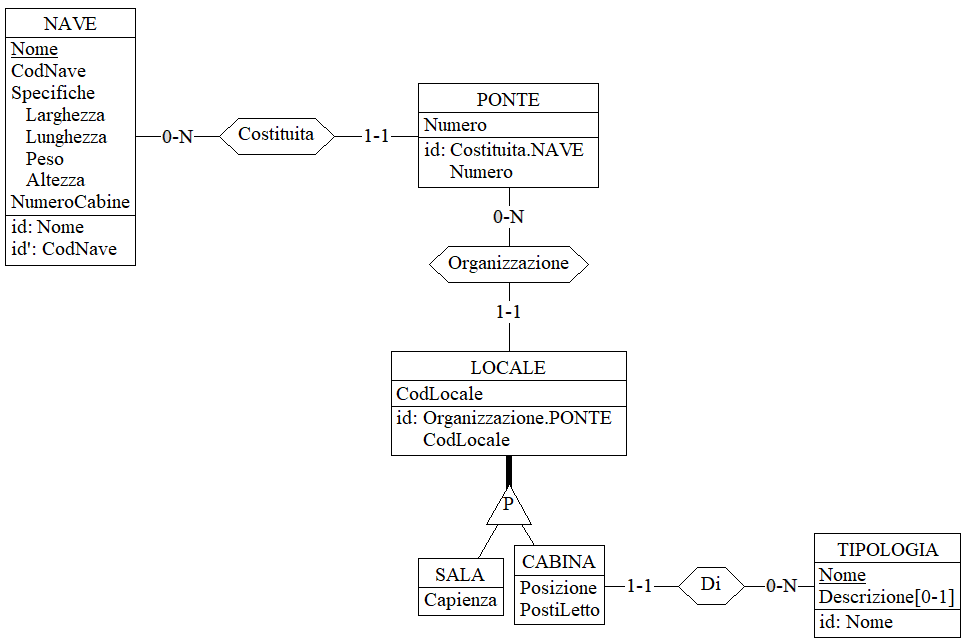
\includegraphics[scale=0.7]{images/Navi.png}		
	\end{figure}	
	\vspace{0.4cm}

	\noindent
	Una nave \textit{può} essere associata ad un \textbf{percorso}. Questa cardinalità minima è dettata dalla necessità di poter creare una nave senza che, obbligatoriamente, le venga associato un relativo percorso. L'entità \textbf{navigazione} descrive la ripetizione dello stesso percorso, ad opera della stessa nave. Si sceglie di definire l'entità \textbf{tratta} che modella staticamente il singolo spostamento, da un porto di partenza ad un porto di arrivo. Si separano, quindi, gli aspetti statici concernenti i percorsi e le \textbf{tratte}, da quelli dinamici riguardanti la loro attivazione ed esecuzione nel tempo, con l'entità \textbf{esecuzioneTratta}. \\	
	Per quanto riguarda gli identificatori di quest'ultima: 
	\begin{itemize}
		\item \textit{il primo identificatore} (Tratta-Navigazione-Partenza.Data) fa sì che non possa essere eseguita la stessa navigazione, lo stesso giorno, per la stessa tratta
		\item \textit{il secondo identificatore} (Navigazione-Data.Arrivo-Ora.Arrivo) impedisce che possano esistere due esecuzioni della stessa navigazione che arrivano in uno stesso giorno ed ora
		\item \textit{il terzo identificatore} (Navigazione-Partenza.Data-Partenza.Ora) fa in modo tale che non possano esistere due esecuzioni della stessa navigazione che partano in un stesso giorno ed ora
	\end{itemize}
	Una navigazione comprende, in generale, più esecuzioni tratte ed è concesso che due navigazioni diverse possano partire/arrivare nello stesso giorno e nella stessa ora. \\
	
	\noindent		
	La struttura ciclica (\textit{nave-percorso-navigazione}), congiuntamente al fatto che ad una nave è associato, al più, ad un percorso, genera il vincolo inespresso che la \textbf{navigazione} effettuata dalla nave esegua il percorso associato alla stessa.\\	
	Inoltre, all'atto della creazione della navigazione è necessario controllare che le date siano consistenti, ovvero che la data-fine sia successiva alla data di inizio e che quest'ultima non sia precedente alla data-fine di una navigazione già esistente.\\	
	Infine, va controllato che il porto di arrivo di una tratta coincida con il porto di partenza della successiva. \\	
	
	\noindent
	Si nota la presenza di una ridondanza dell'attributo numero di esecuzioni, nell'associazione \textbf{esecuzione}, in quanto derivabile da Navigazione e Percorso.
	
    \vspace{0.4cm}
	\begin{figure}[h]
		\centering
		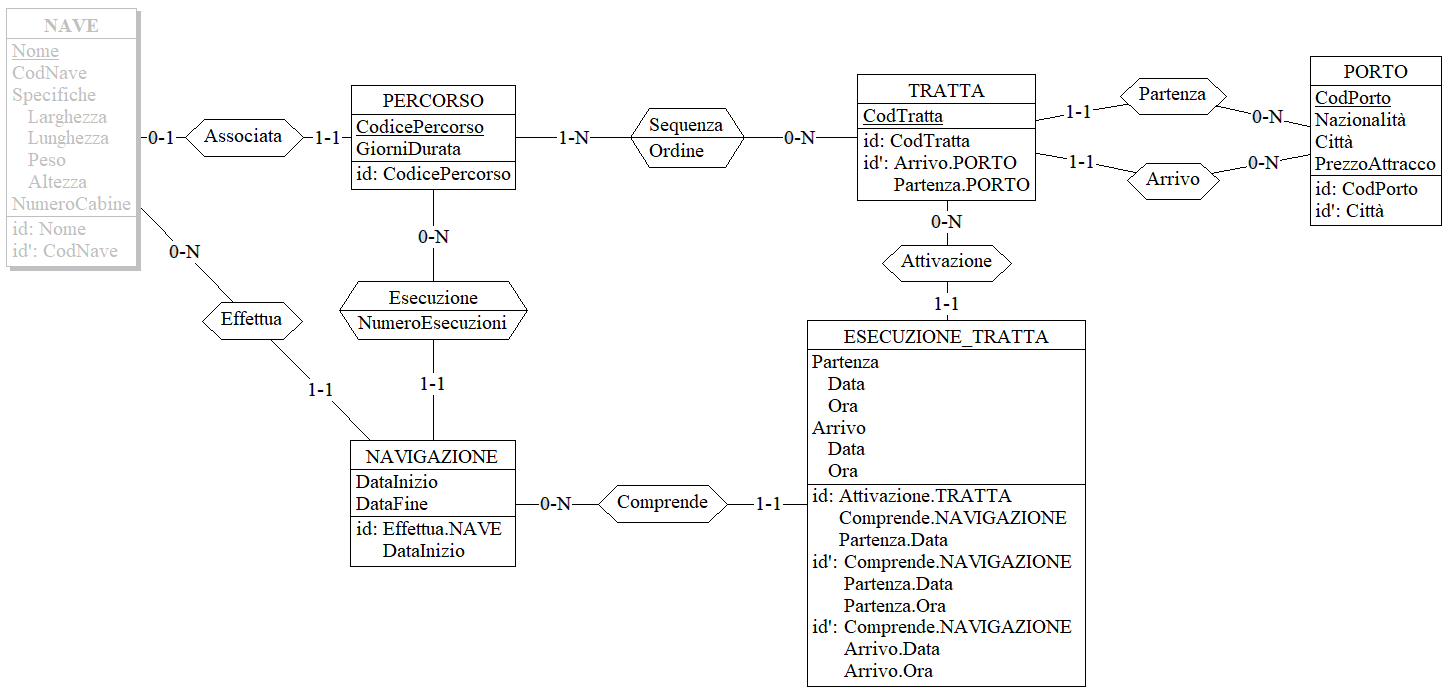
\includegraphics[scale=0.55]{images/Navigazione.png}		
	\end{figure}
	\vspace{0.4cm}
	\noindent
	L'entità \textbf{personale} e \textbf{passeggero} sono la generalizzazione dell'entità \textbf{persona}, che viene identificata dal Codice Fiscale, per evitare problemi di omocodia; vengono inoltre descritte le generalità comuni sia ai passeggeri che la personale. \\ Il personale viene studiato su diversi piani: 
	\begin{itemize}
		\item a livello dei \textbf{turni lavorativi} si sceglie di identificare questa entità con \texttt{(Personale, DataOraInizio)}, con attenzione riposta sui vincoli inespressi
			\begin{enumerate}
			\item La fine del turno deve essere successiva all'inizio dello stesso;
			\item La data di inizio del turno lavorativo deve essere coerente con la navigazione; 
			\item Non possono essere svolti più turni contemporaneamente dallo stesso personale. 
			\end{enumerate}
		\item a livello di \textbf{ruoli} si specifica che ogni impiegato è specializzato in un solo ruolo e può prestare servizio in diverse navigazioni. Si tiene traccia dello storico di ciascun ruolo di responsabilità assunto per ogni  navigazione. Dall'analisi dei requisiti è emersa la necessità di determinare il responsabile, dato un ruolo e una navigazione; da ciò deriva la sua identificazione esterna e l'associazione \texttt{ResponsabilitàPersonale}. 
		\item a livello di composizione, in quanto suddiviso tra la parte \textbf{civile} e l'\textbf{equipaggio} marittimo.
	\end{itemize}
	
	Si noti inoltre che dallo schema emerge il seguente vincolo inespresso: un personale non può essere responsabile all’interno di una navigazione se non vi presta servizio.
	
    \noindent	
	\begin{figure}[h]
		\centering
		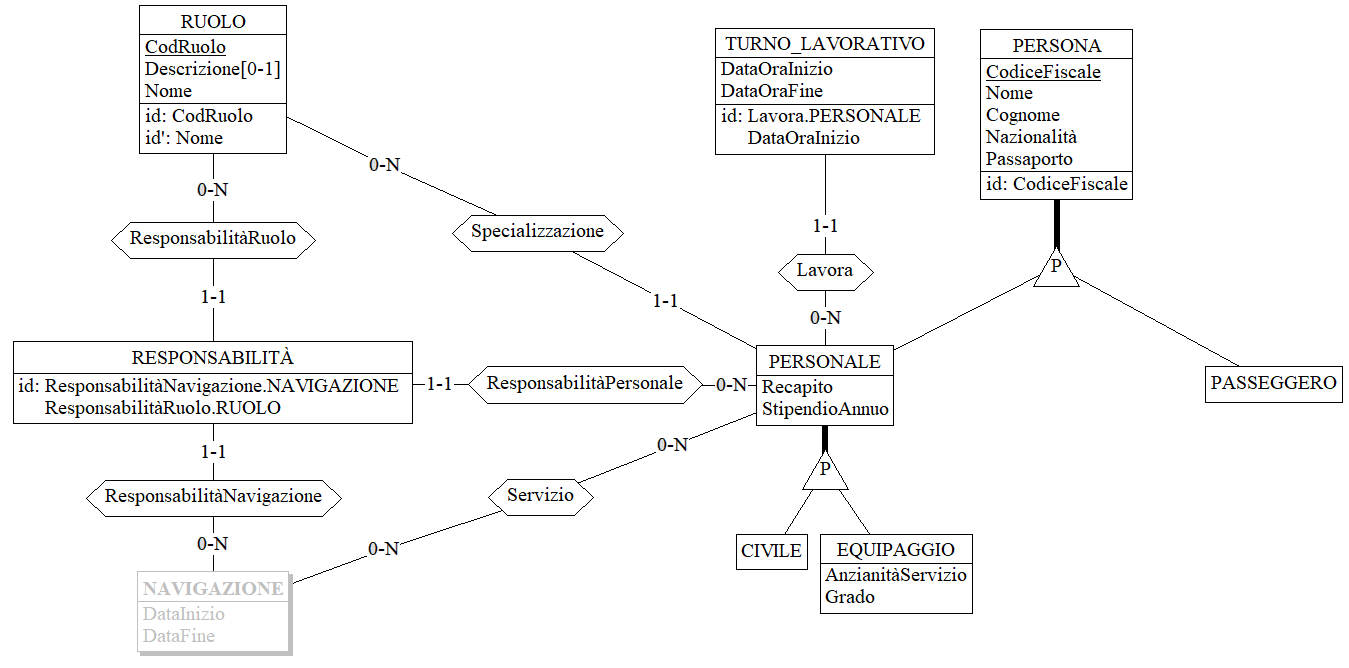
\includegraphics[scale=0.6]{images/Personale.png}		
	\end{figure}
    \vspace{0.6cm}
\newpage

	\noindent
	Le \textbf{attività}, svolte all'interno di una navigazione, vengono svolte in diversi orari e diverse sale.
	L'entità \textbf{attività}, identificata da un codice, viene dinamicamente modellata da \textbf{programmazione}. Gli identificatori di quest'ultima sono stati definiti in modo tale che:
	\begin{itemize}
		\item non sia possibile che all'interno della stessa navigazione, vi siano contemporaneamente due attività nello stesso momento, nella stessa sala;
		\item si determinano ora e durata dell'intrattenimento, conoscendo l'attività, la sala e la navigazione.
	\end{itemize} 
	 \vspace{0.4cm}
	 \begin{figure}[h]
		\centering
		\includegraphics[scale=0.65]{images/Attività.png}		
	\end{figure}
    \vspace{0.6cm}
    
	\noindent
	La \textbf{prenotazione} è l'entità che funge da collegamento per tutti gli schemi definiti fino ad ora. Si modella che una prenotazione, identificata da codice, possa comprendere più passeggeri, in modo tale da consentire la prenotazione per gruppi o per famiglie. Ogni singolo passeggero sarà, però, munito di un \textbf{badge},  che consentirà l'identificazione dello stesso. Viene considerata la possibilità che un passeggero possa effettuare diverse prenotazioni alle quali è associato ogni volta un badge diverso. Tramite l'uso del badge, il passeggero può effettuare delle \texttt{Spese Extra} per acquistare beni o servizi messi a disposizione dalla nave, motivo per cui viene associata una carta di credito che non viene usata come identificatore in quanto può essere la stessa anche per badge diversi, ricordando che una prenotazione può includere delle famiglie. \\
	
	\noindent
	La prenotazione è associata ad un porto ed assume implicitamente che il porto di imbarco sia lo stesso dello sbarco, in cui terminerà il soggiorno. \\
	
	\noindent
	Una prenotazione è associata a una o più cabine, anche di tipologie differenti. La gestione dei prezzi è a carico del \textbf{tariffario}, che vincola i prezzi riguardanti una nave e la tipologia della cabina, relativamente ad un arco temporale, dando così la possibilità al committente di inserire diverse fasce di prezzo in base alla stagione che si prospetta. \\
	\noindent
	Per quanto riguarda i pagamenti previsti per la prenotazione vengono modellati in modo tale da garantire due soluzioni per il pagamento, \textbf{unico} e \textbf{rateizzato}, il quale prevederà il pagamento di alcune \textbf{rate}.\\

	\noindent
	Si evidenziano i seguenti vincoli inespressi inespressi:
	\begin{itemize}
		\item vi siano "accavallamenti" di prenotazioni sulla stessa cabina durante l'intervallo DataImbarco - DataSbarco
		\item Non possono esserci due prenotazioni distinte inerenti allo stesso passeggero nello stesso periodo;
		\item la somma dei posti letto associati ad una prenotazione deve essere maggiore o uguale al numero di passeggeri della prenotazione stessa;
	    \item Il tariffario associato ad una prenotazione deve essere coerente con la tipologia delle cabine della prenotazione.
        \item Il tariffario associato ad una prenotazione deve essere coerente con la nave della prenotazione.
	\end{itemize}
	
		\begin{figure}[h]
		\centering
		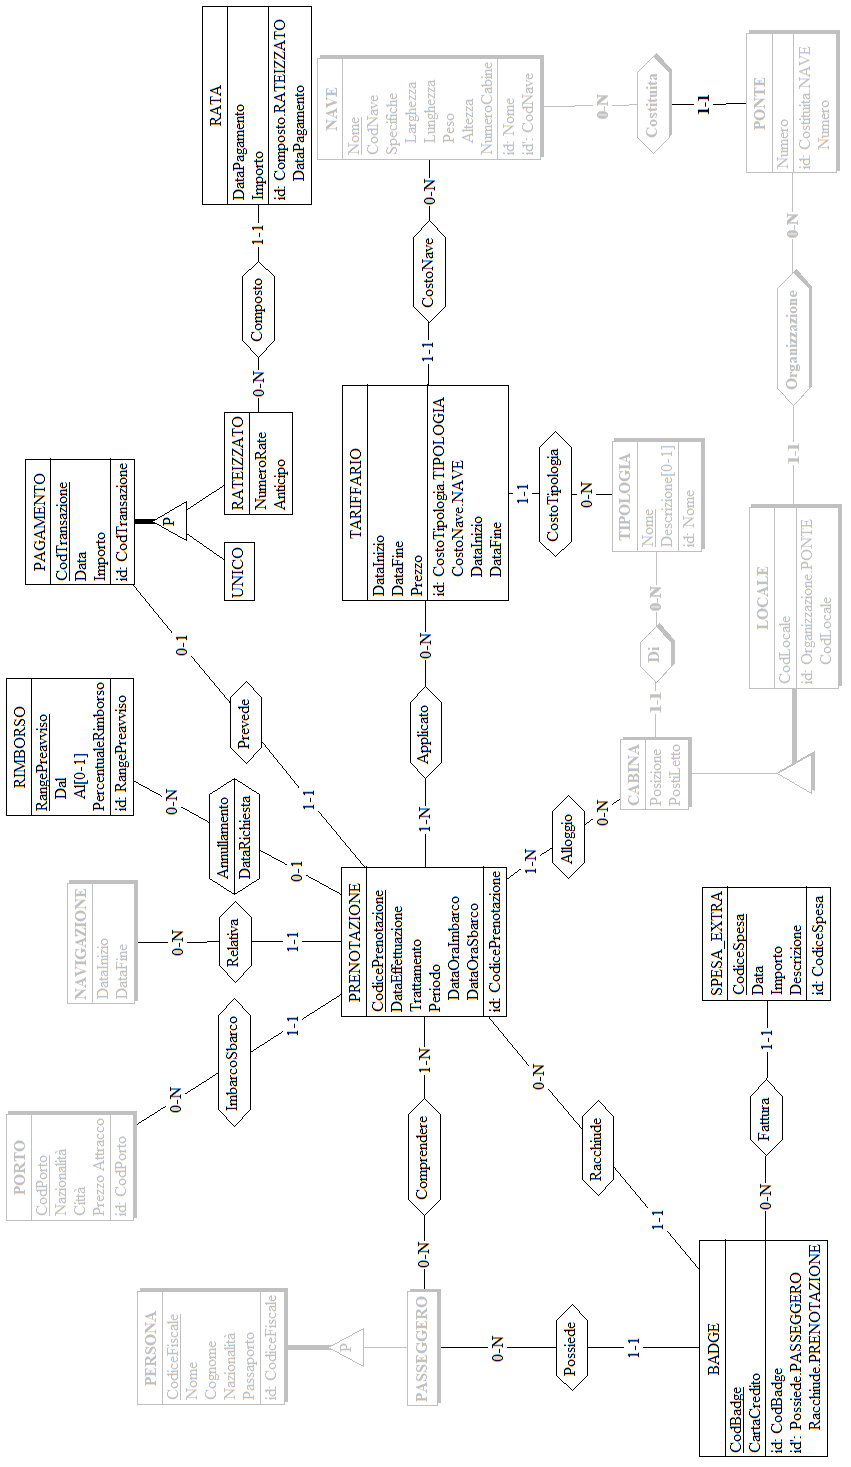
\includegraphics[scale=0.65]{images/Prenotazione.png}		
	\end{figure}


\newpage
\addcontentsline{toc}{section}{Schema generale}	
	\begin{figure}[h!]
		\centering
		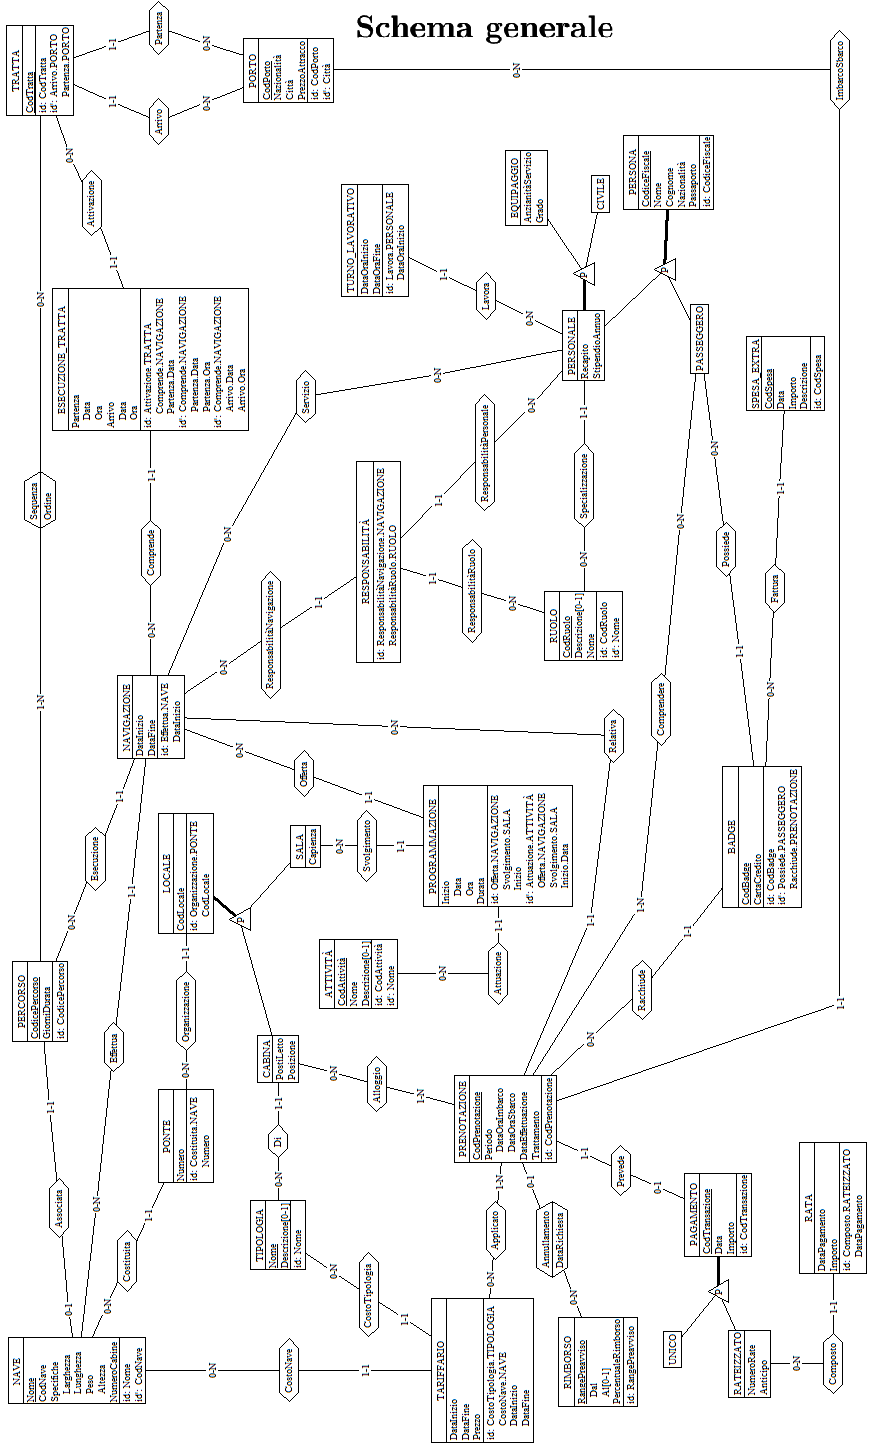
\includegraphics[scale=0.87]{images/SchemaCompl01.png}		
	\end{figure}


\chapter*{\centering{Progettazione logica}}	
\addcontentsline{toc}{chapter}{Progettazione logica}

\section*{Stima del volume dei dati}
\addcontentsline{toc}{section}{Stima del volume dei dati}		

	\begin{figure}[h]
		\centering
		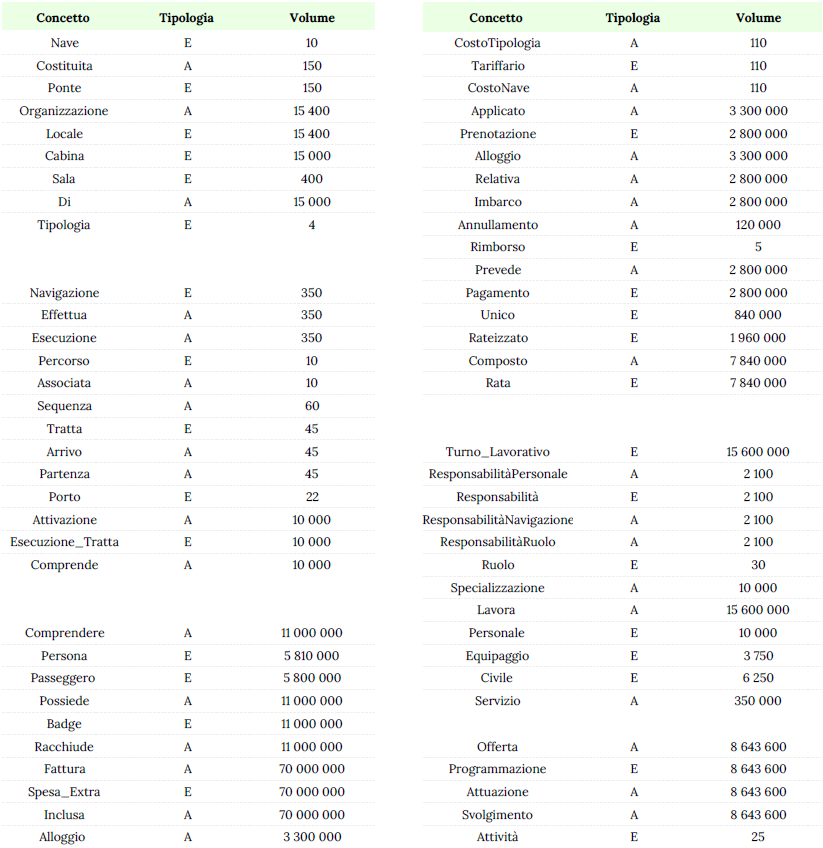
\includegraphics[scale=1]{images/TabVolumi.png}		
	\end{figure}	
	

\newpage


\section*{Descrizione delle operazioni principali e stima della loro frequenza}
\addcontentsline{toc}{section}{Descrizione delle operazioni principali e stima della loro frequenza}	

Segue una tabella con le frequenze delle principali operazioni richieste dal committente:

	\begin{figure}[h]
		\centering
		\arrayrulecolor{GreenYellow}
		\begin{tabular}{c c c}
			\rowcolor{GreenYellow}
			\rule[-6mm]{0mm}{1.5cm}
			\textbf{Codice} & \textbf{Operazione} &\textbf{Frequenza} \\
			\hline
			\rule[-4mm]{0mm}{1cm}		
			1 & \quantities{Inserimento di una prenotazione} & 350 al giorno \\
			\hline
			\rule[-4mm]{0mm}{1cm}
			2 & \quantities{Inserimento nuova navigazione} & 45 all'anno  \\
			\hline
			\rule[-4mm]{0mm}{1cm}
			3 & \quantities{Inserimento di una nuova nave} & 1 ogni 4 anni \\
			\hline
			\rule[-4mm]{0mm}{1cm}
			4 & \quantities{Inserimento di Spesa Extra} & 27 500 al giorno \\
			\hline
			\rule[-4mm]{0mm}{1cm}
			5 & \quantities{Visualizzazione delle navigazioni associate\\ ad una nave} & 1000 al giorno \\
			\hline
			\rule[-4mm]{0mm}{1cm}
			6 & \quantities{Visualizzazione dell'esecuzione tratta \\ all'interno di una navigazione} & 1000 al giorno\\
			\hline
			\rule[-4mm]{0mm}{1cm}
			7 & \quantities{Visualizzazione del percorso e delle \\relative tratte associate ad una nave} & 1000 al giorno\\
			\hline
			\rule[-4mm]{0mm}{1cm}
			8 & \quantities{Visualizzazione della programmazioni relative \\ad una navigazione} & 10 a settimana \\
			\hline
			\rule[-4mm]{0mm}{1cm}
			9 & \quantities{Visualizzazione delle responsabilità \\ relative ad una navigazione} & 6 al mese \\
			\hline
			\rule[-4mm]{0mm}{1cm}
			10 & \quantities{Visualizzazione dei turni lavorativi di \\un personale all'interno di una navigazione } & 800 ogni due settimane \\
			\hline
			\rule[-4mm]{0mm}{1cm}
			11 & \quantities{Visualizzazione del personale con \\più responsabilità } & 6 al mese \\
			\hline
			\rule[-4mm]{0mm}{1cm}
			12 &\quantities{Percorsi più apprezzati} & 2 all'anno \\
			\hline
			\rule[-4mm]{0mm}{1cm}
			13 & \quantities{Costo medio delle prenotazioni per ciascun percorso} & 2 all'anno \\
			\hline
			\rule[-4mm]{0mm}{1cm}
			14 & \quantities{Incassi lordi dell'ultimo anno} & 1 all'anno \\
			\hline
			\rule[-4mm]{0mm}{1cm}
			15 & \quantities{Porti con più imbarchi} & 2 all'anno \\
			\hline
			\rule[-4mm]{0mm}{1cm}
			16 & \quantities{Visualizzazione del tariffario di una nave} & 700 al giorno \\
			\hline
			\rule[-4mm]{0mm}{1cm}
			17 & Inserimento di un nuovo percorso & 1 ogni 4 anni \\
			\hline
		\end{tabular}
	\end{figure}


\newpage

\section*{Schemi di navigazione e tabelle degli accessi }
\addcontentsline{toc}{section}{Schemi di navigazione e tabelle degli accessi }	
\vspace{2cm}
\textbf{{\large Operazione 1:} Inserimento di una prenotazione}\\
\vspace{0.3cm}

\noindent
    L'inserimento di una nuova prenotazione deve tenere conto che sia inserito un badge per ogni passeggero (in media ve ne sono 4 per ogni prenotazione) e che sia letto il numero di cabine sulla nave, in modo tale da verificarne la disponibilità. Bisogna, inoltre, reperire il prezzo della prenotazione e l'inserimento di un nuovo pagamento. \\
    \vspace{0.5cm}
	\begin{figure}[h]
		\centering
		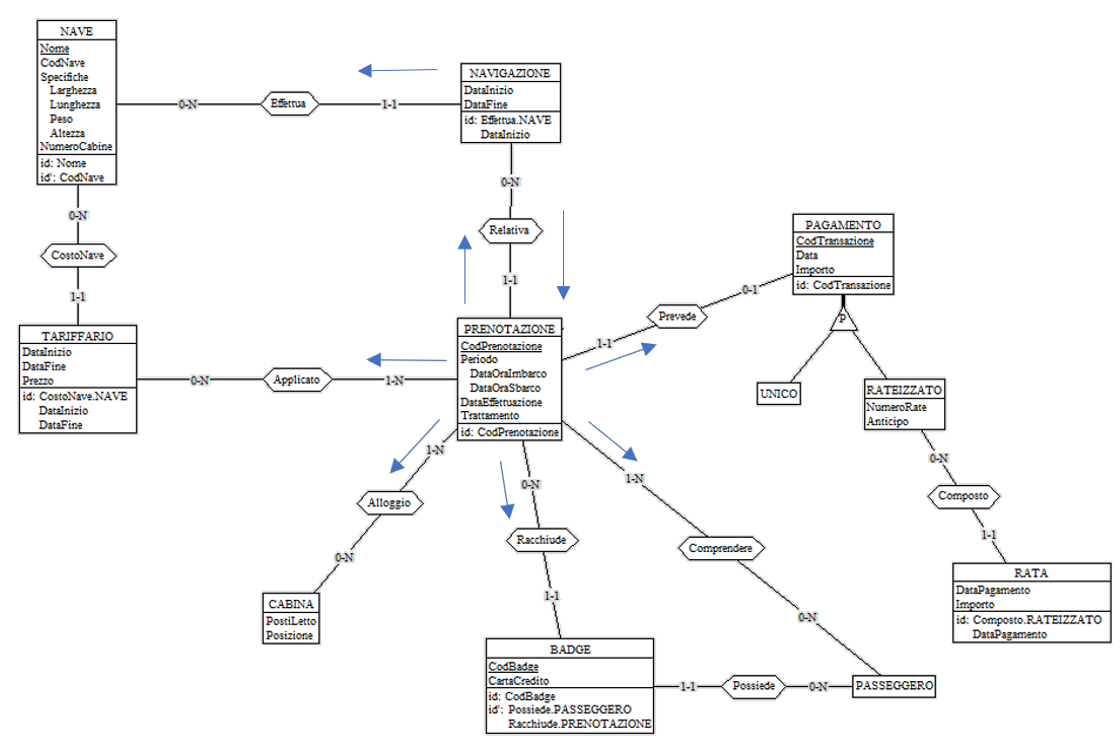
\includegraphics[scale=0.7]{images/SchNav01.png}		
	\end{figure}

   \newpage 
 \begin{figure}[h]
		\centering
		Operazione 1\\
		\arrayrulecolor{GreenYellow}
		\begin{tabular}{L{3cm}C{2.5cm}C{4.5cm}C{2.5cm}}
			\rowcolor{GreenYellow}\rule[-2mm]{0mm}{0.65cm}{}
			\textbf{Concetto} & \textbf{Costrutto} &\textbf{Accessi} & \textbf{Tipo} \\
			\hline
			\rule[-2mm]{0mm}{0.65cm}{}
			Comprendere & A & 11 000 000 / 2 800 000 = 4 & S \\
			\hline
			\rule[-2mm]{0mm}{0.65cm}{}
			Passeggero & E & 11 000 000 / 2 800 000 = 4 & S \\
			\hline
			\rule[-2mm]{0mm}{0.65cm}{}
			Racchiude & A & 11 000 000 / 2 800 000 = 4 & S \\
			\hline
			\rule[-2mm]{0mm}{0.65cm}{}
			Badge & E & 11 000 000 / 2 800 000 = 4 & S \\
			\hline
			\rule[-2mm]{0mm}{0.65cm}{}
			Possiede & E & 11 000 000 / 2 800 000 = 4 & S \\
			\hline
			\rule[-2mm]{0mm}{0.65cm}{}
			Relativa & A & 1 & L \\
			\hline
			\rule[-2mm]{0mm}{0.65cm}{}
			Navigazione & E & 1 & L \\
			\hline
			\rule[-2mm]{0mm}{0.65cm}{}
			Effettua & A & 1 & L \\
			\hline
			\rule[-2mm]{0mm}{0.65cm}{}
			Nave & E & 1 & L \\
			\hline
			\rule[-2mm]{0mm}{0.65cm}{}
			Relativa & A & 2 800 000 / 350 = 8 000 & L \\
			\hline
			\rule[-2mm]{0mm}{0.65cm}{}
			Prenotazione & E & 2 800 000 / 350 = 8 000 & L \\
			\hline
			\rule[-2mm]{0mm}{0.65cm}{}
			Alloggio & A & (3 300 000 / 2 800 000) $\cdot$ 8 000 = 9 600 & L \\
			\hline
			\rule[-2mm]{0mm}{0.65cm}{}
			Cabina & E & (3 300 000 / 2 800 000) $\cdot$ 8 000 = 9 600 & L \\
			\hline
			\rule[-2mm]{0mm}{0.65cm}{}
            Applicato & A & 3 300 000 / 2 800 000 = 1,2 & L \\
            \hline
            \rule[-2mm]{0mm}{0.65cm}{}
            Tariffario & E & 3 300 000 / 2 800 000 = 1,2 & L \\
            \hline
            \rule[-2mm]{0mm}{0.65cm}{}
			Pagamento & E & 1 & S \\
			\hline
			\rule[-2mm]{0mm}{0.65cm}{}
			Prevede & A & 1 & S \\
            \hline\rule[-2mm]{0mm}{0.65cm}{}
			Prenotazione & E & 1 & S \\
		\end{tabular}
		\begin{tabular}{C{13.9cm}}
			\rule[-4mm]{0mm}{1cm}{}	
			\cellcolor{GreenYellow} \textbf{Totale:} 23 S + 35 206 L $\to$ 12 338 340 accessi al giorno
		\end{tabular}
	\end{figure}

\vspace{2cm}
\noindent
\textbf{{\large Operazione 2:}  Inserimento nuova navigazione}\\

\noindent
Per l'inserimento di una nuova navigazione è necessario controllare che  non vi siano navigazioni per quella nave che si sovrappongono con la navigazione che si vuole inserire.
	
	\begin{figure}[h!]
		\centering
		Operazione 2\\
		\arrayrulecolor{GreenYellow}
		\begin{tabular}{L{3cm}C{2.5cm}C{4.5cm}C{2.5cm}}
			\rowcolor{GreenYellow}\rule[-2mm]{0mm}{0.65cm}{}
			\textbf{Concetto} & \textbf{Costrutto} &\textbf{Accessi} & \textbf{Tipo} \\
			\hline\rule[-2mm]{0mm}{0.65cm}{}
			Navigazione & E & 1 & S \\
			\hline\rule[-2mm]{0mm}{0.65cm}{}
			Navigazione & E & 350/10 = 35 & L \\
			\hline\rule[-2mm]{0mm}{0.65cm}{}
            Effettua & A & 1 & S \\
			\hline\rule[-2mm]{0mm}{0.65cm}{}
            Esecuzione& A & 1 & S\\
		\end{tabular}
		\begin{tabular}{C{13.9cm}}
			\rule[-4mm]{0mm}{1cm}{}	
			\cellcolor{GreenYellow} \textbf{Totale:} 35 L + 3 S $\to$ 1 845 accessi all'anno
		\end{tabular}
	\end{figure}
	

\newpage
\noindent
\textbf{{\large Operazione 3:} Inserimento di una nuova nave} \\

	\begin{figure}[h!]
		\centering
		Operazione 3 \\
		\arrayrulecolor{GreenYellow}
		\begin{tabular}{L{3cm}C{2.5cm}C{4.5cm}C{2.5cm}}
			\rowcolor{GreenYellow}\rule[-2mm]{0mm}{0.65cm}{}
			\textbf{Concetto} & \textbf{Costrutto} &\textbf{Accessi} & \textbf{Tipo} \\
			\hline\rule[-2mm]{0mm}{0.65cm}{}
			Nave & E & 1 & S \\
		\end{tabular}
		\begin{tabular}{C{13.9cm}}
			\rule[-4mm]{0mm}{1cm}{}	
			\cellcolor{GreenYellow} \textbf{Totale:} 1 S $\to$ 2 accessi ogni 4 anni
		\end{tabular}
	\end{figure}

\vspace{1cm}
\noindent
\textbf{\large{Operazione 4:} }\textbf{Inserimento di Spesa Extra}
	
	\begin{figure}[h]
		\centering
		Operazione 4 \\
		\arrayrulecolor{GreenYellow}
		\begin{tabular}{L{3cm}C{2.5cm}C{4.5cm}C{2.5cm}}
			\rowcolor{GreenYellow}\rule[-2mm]{0mm}{0.65cm}{}
			\textbf{Concetto} & \textbf{Costrutto} &\textbf{Accessi} & \textbf{Tipo} \\
			\hline\rule[-2mm]{0mm}{0.65cm}{}
			Spesa Extra & E & 1 & S \\
			\hline\rule[-2mm]{0mm}{0.65cm}{}
			Fattura & A & 1 & S \\
		\end{tabular}
		\begin{tabular}{C{13.9cm}}
			\rule[-4mm]{0mm}{1cm}{}	
			\cellcolor{GreenYellow} \textbf{Totale:} 2 S $\to$ 110.000 accessi al giorno.
		\end{tabular}
	\end{figure}

\vspace{1cm}
\noindent
\textbf{\large{Operazione 5: }}\textbf{Visualizzazione delle navigazioni associate ad una nave}

	\begin{figure}[h!]
		\centering
		Operazione 5\\
		\arrayrulecolor{GreenYellow}
		\begin{tabular}{L{3cm}C{2.5cm}C{4.5cm}C{2.5cm}}
			\rowcolor{GreenYellow}\rule[-2mm]{0mm}{0.65cm}{}
			\textbf{Concetto} & \textbf{Costrutto} &\textbf{Accessi} & \textbf{Tipo} \\
			\hline\rule[-2mm]{0mm}{0.65cm}{}
			Effettua & A & 35 & L \\
			\hline\rule[-2mm]{0mm}{0.65cm}{}
			Navigazione & E & 35 & L \\
		\end{tabular}
		\begin{tabular}{C{13.9cm}}
			\rule[-4mm]{0mm}{1cm}{}	
			\cellcolor{GreenYellow} \textbf{Totale:} 70 L $\to$ 70.000 accessi al giorno
		\end{tabular}
	\end{figure}

\vspace{1cm}
\noindent
\textbf{\large {Operazione 6: }}\textbf{Visualizzazione dell'esecuzione tratta all’interno di una navigazione}\\
Per la visualizzazione dell'esecuzione tratta si suppone il codice di navigazione sia dato.
	\begin{figure}[h!]
		\centering
		Operazione 6 \\
		\arrayrulecolor{GreenYellow}
		\begin{tabular}{L{3cm}C{2.5cm}C{4.5cm}C{2.5cm}}
			\rowcolor{GreenYellow}\rule[-2mm]{0mm}{0.65cm}{}
			\textbf{Concetto} & \textbf{Costrutto} &\textbf{Accessi} & \textbf{Tipo} \\
			\hline\rule[-2mm]{0mm}{0.65cm}{}
			Comprende & A & 10 000 / 350 = 28,6  & L \\
			\hline\rule[-2mm]{0mm}{0.65cm}{}
			Esecuzione Tratta & E & 10 000 / 350 = 28.6  & L \\
		\end{tabular}
		\begin{tabular}{C{13.9cm}}
			\rule[-4mm]{0mm}{1cm}{}	
			\cellcolor{GreenYellow} \textbf{Totale:} 57 L $\to$ 57 000 accessi al giorno
		\end{tabular}
	\end{figure}

\newpage
\noindent
\textbf{{\large {Operazione 7: }}}\textbf{Visualizzazione del percorso e delle relative tratte associate ad una nave}

	  \vspace{0.5cm}
	\begin{figure}[h]
		\centering
		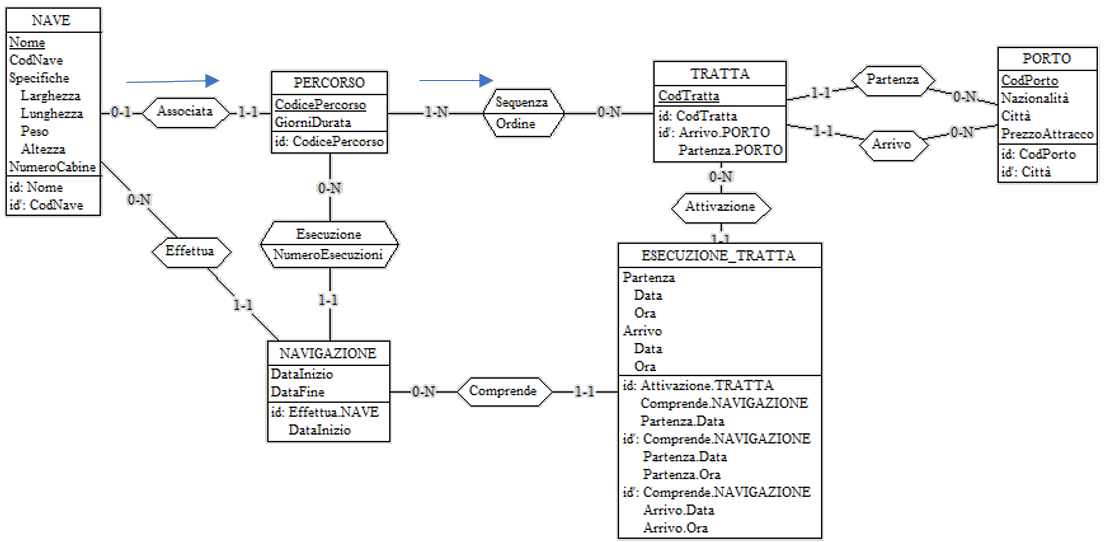
\includegraphics[scale=0.7]{images/SchNav02.png}		
	\end{figure}
	\vspace{0.5cm}
	\begin{figure}[h]
		\centering
		Operazione 7\\
		\arrayrulecolor{GreenYellow}
		\begin{tabular}{L{3cm}C{2.5cm}C{4.5cm}C{2.5cm}}
			\rowcolor{GreenYellow}\rule[-2mm]{0mm}{0.65cm}{}
			\textbf{Concetto} & \textbf{Costrutto} &\textbf{Accessi} & \textbf{Tipo} \\
			\hline\rule[-2mm]{0mm}{0.65cm}{}
			Associata & A & 1 & L \\
			\hline\rule[-2mm]{0mm}{0.65cm}{}
			Percorso & E & 1 & L \\
			\hline\rule[-2mm]{0mm}{0.65cm}{}
			Sequenza & A & 60 / 10 = 6 & L \\
			\hline\rule[-2mm]{0mm}{0.65cm}{}
			Tratta & E & 60 / 10 = 6 & L \\
		\end{tabular}
		\begin{tabular}{C{13.9cm}}
			\rule[-4mm]{0mm}{1cm}{}	
			\cellcolor{GreenYellow} \textbf{Totale:} 14 L $\to$ 14 000 accessi al giorno
		\end{tabular}
	\end{figure}
	
	\vspace{2cm}
	
\noindent
\textbf{{\large {Operazione 8: }}}\textbf{Visualizzazione delle programmazioni in una navigazione}

	
	
	\begin{figure}[h]
		\centering
		Operazione 8\\
		\arrayrulecolor{GreenYellow}
		\begin{tabular}{L{3cm}C{2.5cm}C{4.5cm}C{2.5cm}}
			\rowcolor{GreenYellow}\rule[-2mm]{0mm}{0.65cm}{}
			\textbf{Concetto} & \textbf{Costrutto} &\textbf{Accessi} & \textbf{Tipo} \\
			\hline\rule[-2mm]{0mm}{0.65cm}{}
			Offerta & A & 8 643 600 / 350 = 24 696 & L \\
			\hline \rule[-2mm]{0mm}{0.65cm}{}
			Programmazione & E & 8 643 600 / 350 = 24 696 & L \\
		\end{tabular}
		\begin{tabular}{C{13.9cm}}
			\rule[-4mm]{0mm}{1cm}{}	
			\cellcolor{GreenYellow} \textbf{Totale:} 49 392 L $\to$ 493 920 accessi a settimana
		\end{tabular}
	\end{figure}
	
	\newpage
	
\noindent
\textbf{{\large {Operazione 9: }}}\textbf{Visualizzazione delle responsabilità di una navigazione}

	
	
	\begin{figure}[h]
		\centering
		Operazione 9\\
		\arrayrulecolor{GreenYellow}
		\begin{tabular}{L{3cm}C{2.5cm}C{4.5cm}C{2.5cm}}
			\rowcolor{GreenYellow}\rule[-2mm]{0mm}{0.65cm}{}
			\textbf{Concetto} & \textbf{Costrutto} &\textbf{Accessi} & \textbf{Tipo} \\
			\hline\rule[-2mm]{0mm}{0.65cm}{}
			Responsabilità Navigazione & A & 2 100 / 350 = 6 & L \\
			\hline \rule[-2mm]{0mm}{0.65cm}{}
			Responsabilità & E & 2 100 / 350 = 6 & L \\
		\end{tabular}
		\begin{tabular}{C{13.9cm}}
			\rule[-4mm]{0mm}{1cm}{}	
			\cellcolor{GreenYellow} \textbf{Totale:} 12 L $\to$ 72  accessi al mese
		\end{tabular}
	\end{figure}
	
	\vspace{0.5cm}
	
	\noindent
	\textbf{{\large {Operazione 10:}}}\textbf{ Visualizzazione dei turni lavorativi di un personale all'interno di una navigazione}
    \noindent
	Supponiamo di avere a disposizione sia la navigazione che il personale.
	
	 \vspace{0.5cm}
	\begin{figure}[h]
		\centering
		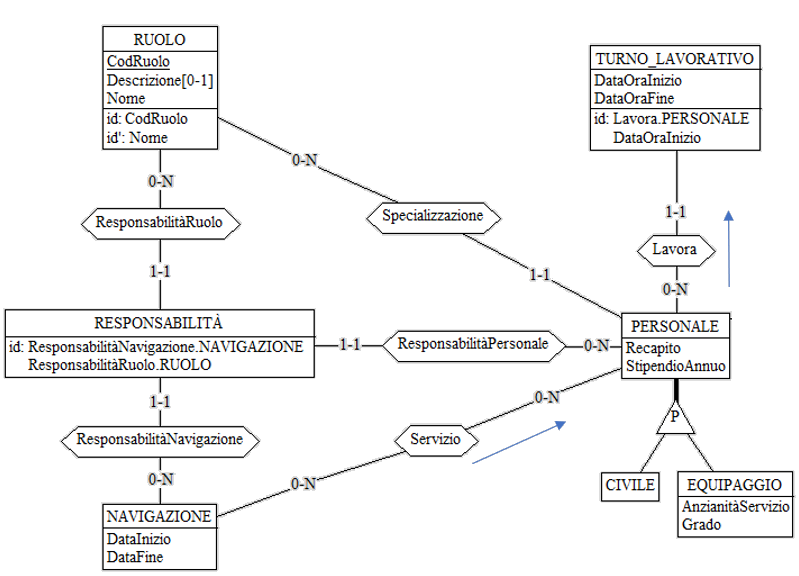
\includegraphics[scale=0.7]{images/SchNav03.png}		
	\end{figure}
	\vspace{0.5cm}
	\begin{figure}[h]
		\centering
		Operazione 10\\
		\arrayrulecolor{GreenYellow}
		\begin{tabular}{L{3cm}C{2.5cm}C{4.5cm}C{2.5cm}}
			\rowcolor{GreenYellow}\rule[-2mm]{0mm}{0.65cm}{}
			\textbf{Concetto} & \textbf{Costrutto} &\textbf{Accessi} & \textbf{Tipo} \\
			\hline\rule[-2mm]{0mm}{0.65cm}{}
			Servizio & A & 350 000 / 350 = 1 000 & L \\
			\hline\rule[-2mm]{0mm}{0.65cm}{}
			Personale & E & 350 000 / 350 = 1 000 & L \\
			\hline\rule[-2mm]{0mm}{0.65cm}{}
			Lavora & A & 15 600 000 / 10 000 = 1 560 & L \\
			\hline\rule[-2mm]{0mm}{0.65cm}{}
			Turno Lavorativo & E & 15 600 000 / 10 000 = 1 560 & L \\
		\end{tabular}
		\begin{tabular}{C{13.9cm}}
			\rule[-4mm]{0mm}{1cm}{}	
			\cellcolor{GreenYellow} \textbf{Totale:} 5120 accessi $\to$ 4 096 000 accessi ogni 2 settimane
		\end{tabular}
	\end{figure}
	

\newpage
	\noindent
	\textbf{{\large {Operazione 11: }}}\textbf{Visualizzazione del personale con più responsabilità}
	 \vspace{0.5cm}
	\begin{figure}[h]
		\centering
		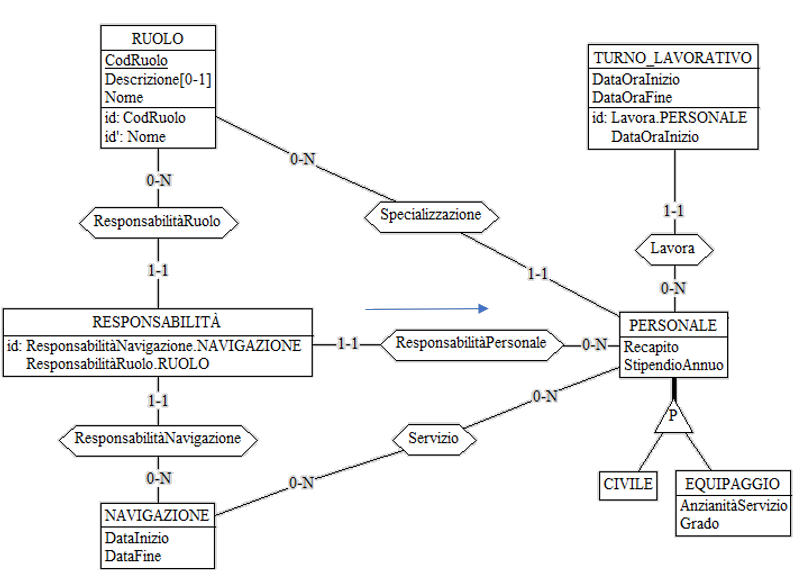
\includegraphics[scale=0.7]{images/SchNav04.png}		
	\end{figure}
	\vspace{0.5cm}
	\begin{figure}[h]
		\centering
		Operazione 11\\
		\arrayrulecolor{GreenYellow}
		\begin{tabular}{L{3cm}C{2.5cm}C{4.5cm}C{2.5cm}}
			\rowcolor{GreenYellow}\rule[-2mm]{0mm}{0.65cm}{}
			\textbf{Concetto} & \textbf{Costrutto} &\textbf{Accessi} & \textbf{Tipo} \\
			\hline\rule[-2mm]{0mm}{0.65cm}{}
			Responsabilità & E & 2.100 & L \\
			\hline\rule[-2mm]{0mm}{0.65cm}{}
			Responsabilità Personale & A & 1 & L \\
			\hline\rule[-2mm]{0mm}{0.65cm}{}
			Personale & E & 1 & L \\
		\end{tabular}
		\begin{tabular}{C{13.9cm}}
			\rule[-4mm]{0mm}{1cm}{}	
			\cellcolor{GreenYellow} \textbf{Totale:} 2 102 accessi $\to$ 12 612 accessi al mese
		\end{tabular}
	\end{figure}
	
\vspace{1cm}
	\noindent
	\textbf{{\large {Operazione 12: }}}\textbf{Percorsi più apprezzati}  \\
	Viene stilata una classifica dei percorsi che hanno avuto più prenotazioni.
	\begin{figure}[h]
		\centering
		Operazione 12 \\
		\arrayrulecolor{GreenYellow}
		\begin{tabular}{L{3cm}C{2.5cm}C{4.5cm}C{2.5cm}}
			\rowcolor{GreenYellow}\rule[-2mm]{0mm}{0.65cm}{}
			\textbf{Concetto} & \textbf{Costrutto} &\textbf{Accessi} & \textbf{Tipo} \\
			\hline\rule[-2mm]{0mm}{0.65cm}{}
			Prenotazioni & E & 2 800 000 & L \\
			\hline\rule[-2mm]{0mm}{0.65cm}{}
			Relativa & A & 1 & L \\
			\hline\rule[-2mm]{0mm}{0.65cm}{}
			Navigazione & E & 1 & L \\
		\end{tabular}
		\begin{tabular}{C{13.9cm}}
			\rule[-4mm]{0mm}{1cm}{}	
			\cellcolor{GreenYellow} \textbf{Totale:} 2.800.002 L $\to$ 466 667 accessi al mese
		\end{tabular}
	\end{figure}
	
	

\newpage
	
	\noindent
	\textbf{{\large {Operazione 13: }}}\textbf{Costo medio delle prenotazioni per ciascun percorso}
		 \vspace{0.5cm}
	\begin{figure}[h]
		\centering
		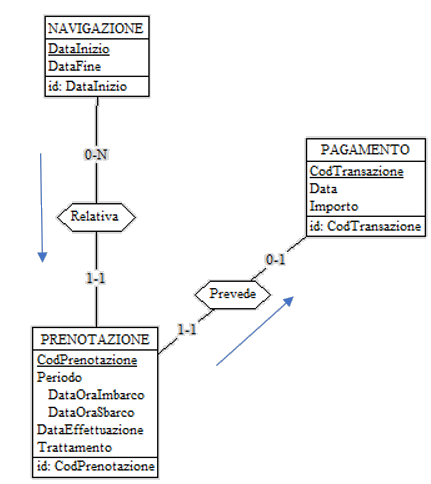
\includegraphics[scale=0.7]{images/SchNav06.png}		
	\end{figure}
	\vspace{0.2cm}
	\begin{figure}[h]
		\centering
		Operazione 13\\
		\arrayrulecolor{GreenYellow}
		\begin{tabular}{L{3cm}C{2.5cm}C{4.5cm}C{2.5cm}}
			\rowcolor{GreenYellow}\rule[-2mm]{0mm}{0.65cm}{}
			\textbf{Concetto} & \textbf{Costrutto} &\textbf{Accessi} & \textbf{Tipo} \\
			\hline\rule[-2mm]{0mm}{0.65cm}{}
			Navigazione & E & 350 & L \\
			\hline\rule[-2mm]{0mm}{0.65cm}{}
			Relativa & A & 2.800.000/350 = 8000 & L \\
			\hline\rule[-2mm]{0mm}{0.65cm}{}
			Prenotazione & E & 2.800.000/350 = 8000 & L \\
			\hline\rule[-2mm]{0mm}{0.65cm}{}
			Prevede & A & 2.800.000/350 = 8000 & L \\
			\hline\rule[-2mm]{0mm}{0.65cm}{}
			Pagamento & E & 2.800.000/350 = 8000 & L \\
		\end{tabular}
		\begin{tabular}{C{13.9cm}}
			\rule[-4mm]{0mm}{1cm}{}	
			\cellcolor{GreenYellow} \textbf{Totale:} 32.350 L $\to$ 5.391 accessi al mese
		\end{tabular}
	\end{figure}
	

	\vspace{0.5cm}
	
	\noindent
	\textbf{{\large {Operazione 14: }}}\textbf{Incassi lordi dell'ultimo anno} \\
    Per incassi lordi si intende la somma dei pagamenti associati ad una navigazione in aggiunta alla totalità delle spese extra effettuate nell'ultimo anno.
	
	\begin{figure}[h]
		\centering
		Operazione 14\\
		\arrayrulecolor{GreenYellow}
		\begin{tabular}{L{3cm}C{2.5cm}C{4.5cm}C{2.5cm}}
			\rowcolor{GreenYellow}\rule[-2mm]{0mm}{0.65cm}{}
			\textbf{Concetto} & \textbf{Costrutto} &\textbf{Accessi} & \textbf{Tipo} \\
			\hline\rule[-2mm]{0mm}{0.65cm}{}
			Pagamenti & E & 2.800.000 & L \\
			\hline\rule[-2mm]{0mm}{0.65cm}{}
			Spese extra & E & 70.000.000 & L \\
		\end{tabular}
		\begin{tabular}{C{13.9cm}}
			\rule[-4mm]{0mm}{1cm}{}	
			\cellcolor{GreenYellow} \textbf{Totale:} 72.800.000 L $\to$ 6 066 666 accessi al mese
		\end{tabular}
	\end{figure}

	\vspace{0.5cm}
	
	\newpage
	
	\noindent
	\textbf{{\large {Operazione 15: }}}\textbf{Porti con più imbarchi}
	\begin{figure}[h!]
		\centering
		Operazione 15 \\
		\arrayrulecolor{GreenYellow}
		\begin{tabular}{L{3cm}C{2.5cm}C{4.5cm}C{2.5cm}}
			\rowcolor{GreenYellow}\rule[-2mm]{0mm}{0.65cm}{}
			\textbf{Concetto} & \textbf{Costrutto} &\textbf{Accessi} & \textbf{Tipo} \\
			\hline\rule[-2mm]{0mm}{0.65cm}{}
			Porto & E & 22 & L \\
			\hline\rule[-2mm]{0mm}{0.65cm}{}
			Imbarco Sbarco & A & 2 800 000 & L \\
		\end{tabular}
		\begin{tabular}{C{13.9cm}}
			\rule[-4mm]{0mm}{1cm}{}	
			\cellcolor{GreenYellow} \textbf{Totale:} 2 800 022 L $\to$ 5 600 044 accessi all'anno
		\end{tabular}
	\end{figure}

	\noindent
	\textbf{{\large{Operazione 16:}}}\textbf{Visualizzazione del tariffario di una nave}
	\vspace{0.5cm}
	\begin{figure}[h]
		\centering
		Operazione 16 \\
		\arrayrulecolor{GreenYellow}
		\begin{tabular}{L{3cm}C{2.5cm}C{4.5cm}C{2.5cm}}
			\rowcolor{GreenYellow}\rule[-2mm]{0mm}{0.65cm}{}
			\textbf{Concetto} & \textbf{Costrutto} &\textbf{Accessi} & \textbf{Tipo} \\
			\hline\rule[-2mm]{0mm}{0.65cm}{}
			Tariffario & E & 110 & L \\
		\end{tabular}
		
		\begin{tabular}{C{13.9cm}}
			\rule[-4mm]{0mm}{1cm}{}	
			\cellcolor{GreenYellow} \textbf{Totale:} 110 L $\to$ 77 000 accessi al mese
		\end{tabular}
	\end{figure}
	
	
	\noindent
	\textbf{{\large {Operazione 17: }}}\textbf{Inserimento di un nuovo percorso}
	  \vspace{0.5cm}
	\begin{figure}[h]
		\centering
		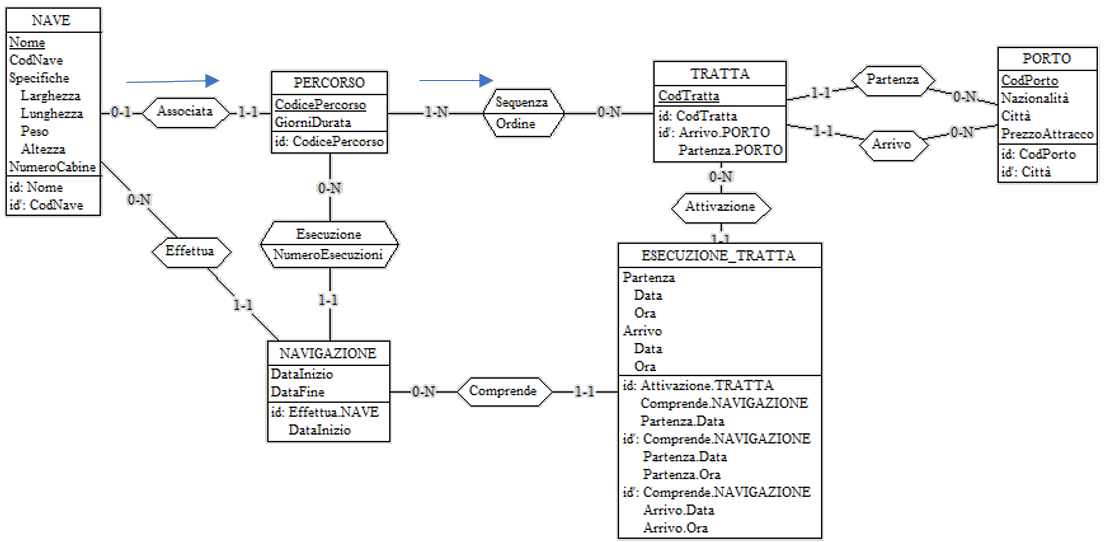
\includegraphics[scale=0.7]{images/SchNav02.png}		
	\end{figure}
	\vspace{0.5cm}
	\begin{figure}[h]
		\centering
		Operazione 17\\
		\arrayrulecolor{GreenYellow}
		\begin{tabular}{L{3cm}C{2.5cm}C{4.5cm}C{2.5cm}}
			\rowcolor{GreenYellow}\rule[-2mm]{0mm}{0.65cm}{}
			\textbf{Concetto} & \textbf{Costrutto} &\textbf{Accessi} & \textbf{Tipo} \\
			\hline\rule[-2mm]{0mm}{0.65cm}{}
			Associata & A & 1 & S \\
			\hline\rule[-2mm]{0mm}{0.65cm}{}
			Sequenza & A & 60/10 = 6 & S \\
			\hline\rule[-2mm]{0mm}{0.65cm}{}
			Percorso & E & 1 & S \\
			\hline\rule[-2mm]{0mm}{0.65cm}{}
			Tratta & E & 6 & L \\
		\end{tabular}
		\begin{tabular}{C{13.9cm}}
			\rule[-4mm]{0mm}{1cm}{}	
			\cellcolor{GreenYellow} \textbf{Totale:} 8 S, 6 L $\to$ 22 accessi ogni 4 anni
		\end{tabular}
	\end{figure}
	


\newpage

\section*{Raffinamento dello schema (eliminazione di identificatori esterni, attributi composti e gerarchie, scelta delle chiavi) }
\addcontentsline{toc}{section}{Raffinamento dello schema}	

\subsection*{Eliminazione delle gerarchie}
Nello schema sono presenti 4 gerarchie di generalizzazione:
\begin{itemize}
    \item \texttt{Locale} con copertura totale ed esclusiva. Si adotta un collasso verso il \textbf{basso} in quanto le operazioni richieste sono specifiche o per le cabine o per le sale e gli accessi sono distinti. Si provvede quindi a spostare gli attributi comuni presenti nell'entità padre nelle due figlie, creando un'associazione con la cabina per ciascuna delle due entità figlie;
    \item \texttt{Persona} con copertura totale ed esclusiva. Si adotta un collasso verso il \textbf{basso} in quanto le operazioni sono specifiche e coinvolgono separatamente il personale e i passeggeri. Come sopra, si spostano gli attributi comuni dell'entità padre nelle due figlie;
    \item \texttt{Personale} con copertura totale ed esclusiva. In questo caso si adotta un collasso verso l'\textbf{alto} in quanto il carico di lavoro è generico e coinvolge allo stesso modo il personale civile e l'equipaggio. Si procede spostando nell'entità padre gli attributi, avendo cura di specificare l'opzionalità degli attributi \texttt{AnzianitàServizio} e \texttt{Grado} caratteristici per l'equipaggio di bordo, ma privi di alcun significato per il personale civile. Inoltre, si definisce un vincolo di coesistenza per i due precedenti attributi: chiaramente o entrambi sono simultaneamente presenti o sono assenti per qualunque istanza. Non è necessario inserire un selettore di tipo in quanto la tipologia del personale è inferibile dalla presenza o meno dei due attributi sopra esposti;
    \item \texttt{Pagamento} con copertura totale ed esclusiva. Si adotta un collasso verso l'\textbf{alto} in quanto gli accessi alle entità padre e figlie sono contestuali. Così come per \texttt{Personale} si spostano gli attributi delle entità figlie in quella padre, specificando le opportune opzionalità e vincoli di coesistenza. 
\end{itemize}

\subsection*{Eliminazione degli attributi composti}
Nello schema sono presenti attributi composti in: \texttt{PROGRAMMAZIONE}, \texttt{ESECUZIONE\_TRATTA}, \texttt{PRENOTAZIONE}, \texttt{RIMBORSO} e \texttt{NAVE}. Per ciascuna di queste entità sono stati opportunamente scomposti i relativi attributi composti.

\subsection*{Scelta delle chiavi primarie}
All'atto della conversione a progetto logico sono stati creati codici identificativi al fine di semplificare i riferimenti ed evitare ambiguità.

\newpage
\section*{Studio delle ridondanze}
\addcontentsline{toc}{section}{Studio delle ridondanze}
\noindent
Si riscontrano due ridondanze all'interno dello schema:
\begin{itemize}
    \item Imbarco/Sbarco, che coinvolge l'operazione 1 e l'operazione 15
    \item NumeroCabine, che coinvolge l'operazione 1 
\end{itemize}
\subsection*{Analisi ridondanza di Imbarco / Sbarco}
Le operazioni che sono coinvolte sono la 1 e la 15: si ipotizza che non ci siano già i passeggeri nel database e che periodo di prenotazione coincida con quello della navigazione \\


\noindent
\textbf{\large{Studio Operazione 1}}\\

    \begin{figure}[h]
		\centering
		Operazione 1 \textit{senza ridondanza}\\
		\arrayrulecolor{GreenYellow}
		\begin{tabular}{L{3cm}C{2.5cm}C{4.5cm}C{2.5cm}}
			\rowcolor{GreenYellow}\rule[-2mm]{0mm}{0.65cm}{}
			\textbf{Concetto} & \textbf{Costrutto} &\textbf{Accessi} & \textbf{Tipo} \\
			\hline\rule[-2mm]{0mm}{0.65cm}{}
			Comprendere & A & 11 000 000 / 2 800 000 = 4 & S \\
			\hline\rule[-2mm]{0mm}{0.65cm}{}
			Passeggero & E & 11 000 000 / 2 800 000 = 4 & S \\
			\hline\rule[-2mm]{0mm}{0.65cm}{}
			Racchiude & A & 11 000 000 / 2 800 000 = 4 & S \\
			\hline\rule[-2mm]{0mm}{0.65cm}{}
			Badge & E & 11 000 000 / 2 800 000 = 4 & S \\
			\hline\rule[-2mm]{0mm}{0.65cm}{}
			Possiede & A & 11 000 000 / 2 800 000 = 4 & S \\
			\hline\rule[-2mm]{0mm}{0.65cm}{}
			Relativa & A & 1 & L \\
			\hline\rule[-2mm]{0mm}{0.65cm}{}
			Navigazione & E & 1 & L \\
			\hline\rule[-2mm]{0mm}{0.65cm}{}
			Effettua & A & 1 & L \\
			\hline\rule[-2mm]{0mm}{0.65cm}{}
			Nave & E & 1 & L \\
			\hline\rule[-2mm]{0mm}{0.65cm}{}
			Relativa & A & 2 800 000 / 350 = 8 000 & L \\
			\hline\rule[-2mm]{0mm}{0.65cm}{}
			Prenotazione & E & 2 800 000 / 350 = 8 000 & L \\
			\hline\rule[-2mm]{0mm}{0.65cm}{}
			Alloggi & A & (3 300 000 / 2 800 000) $\cdot$ 8 000 = 9 600 & L \\
			\hline\rule[-2mm]{0mm}{0.65cm}{}
			Cabina & E & (3 300 000 / 2 800 000) $\cdot$ 8 000 = 9 600 & L \\
			\hline\rule[-2mm]{0mm}{0.65cm}{}
            Applicato & A & 3 300 000 / 2 800 000 = 1,2 & L \\
            \hline\rule[-2mm]{0mm}{0.65cm}{}
            Tariffario & E & 3 300 000 / 2 800 000 = 1,2 & L \\
            \hline\rule[-2mm]{0mm}{0.65cm}{}
			Pagamento & E & 1 & S \\
			\hline\rule[-2mm]{0mm}{0.65cm}{}
			Prevede & A & 1 & S \\
            \hline\rule[-2mm]{0mm}{0.65cm}{}
			Prenotazione & E & 1 & S \\
		\end{tabular}
		\begin{tabular}{C{13.9cm}}
			\rule[-4mm]{0mm}{1cm}{}	
			\cellcolor{GreenYellow} \textbf{Totale:} 23 S + 35206 L $\to$ 12 338 340 al giorno
		\end{tabular}
	\end{figure}
	
	\noindent
	L'\textbf{Operazione 1}\textit{ con ridondanza} ha lo stesso costo di quella senza ridondanza, ma con l'aggiunta di una scrittura per ImbarcoSbarco. Da cui: \\ \textbf{Totale} 24 S + 35206 L $\to $ 12 338 900 accessi al giorno

\newpage
\noindent
\textbf{\large{Studio Operazione 15}}
    \begin{figure}[h]
		\centering
		Operazione 15 \textit{senza ridondanza}\\
		\arrayrulecolor{GreenYellow}
		\begin{tabular}{L{3cm}C{2.5cm}C{4.5cm}C{2.5cm}}
			\rowcolor{GreenYellow}\rule[-2mm]{0mm}{0.65cm}{}
			\textbf{Concetto} & \textbf{Costrutto} &\textbf{Accessi} & \textbf{Tipo} \\
			\hline\rule[-2mm]{0mm}{0.65cm}{}
			Porto & E & 22 & L \\
			\hline\rule[-2mm]{0mm}{0.65cm}{}
			Partenza & A & 45 & L \\
			\hline\rule[-2mm]{0mm}{0.65cm}{}
			Tratta & E & 45 & L \\
			\hline\rule[-2mm]{0mm}{0.65cm}{}	
			Attivazione & A & 10 000 & L \\
			\hline\rule[-2mm]{0mm}{0.65cm}{}
			Esecuzione Tratta & E & 10 000 & L \\
			\hline\rule[-2mm]{0mm}{0.65cm}{}
			Comprende & A & 10 000 & L \\
			\hline\rule[-2mm]{0mm}{0.65cm}{}
			Navigazione & E & 10 000 & L \\
			\hline\rule[-2mm]{0mm}{0.65cm}{}
			Relativa & A & 2 800 000 / 350 $\cdot$ 10.000 = 80 mln & L \\
			\hline\rule[-2mm]{0mm}{0.65cm}{}
			Prenotazione & E & 2 800 000 / 350 $\cdot$ 10.000 = 80 mln & L \\
		\end{tabular}
		\begin{tabular}{C{13.9cm}}
			\rule[-4mm]{0mm}{1cm}{}	
			\cellcolor{GreenYellow} \textbf{Totale:} 160 040 112 L $\to$ 320 080 224 accessi all'anno
		\end{tabular}
	\end{figure}
	
	\begin{figure}[h]
		\centering
		Operazione 15 \textit{con ridondanza}\\
		\arrayrulecolor{GreenYellow}
		\begin{tabular}{C{3cm}C{2.5cm}C{4.5cm}C{2.5cm}}
			\rowcolor{GreenYellow}\rule[-2mm]{0mm}{0.65cm}{}
			\textbf{Concetto} & \textbf{Costrutto} &\textbf{Accessi} & \textbf{Tipo} \\
			\hline\rule[-2mm]{0mm}{0.65cm}{}
			Porto & E & 22 & L \\
			\hline\rule[-2mm]{0mm}{0.65cm}{}
			Imbarco Sbarco & A & 2 800 000 & L \\
		\end{tabular}
		\begin{tabular}{C{13.9cm}}
			\rule[-4mm]{0mm}{1cm}{}	
			\cellcolor{GreenYellow} \textbf{Totale:} 2 800 022 L $\to$ 5 600 044 accessi all'anno
		\end{tabular}
	\end{figure}

\noindent
Data l'analisi conviene mantenere la ridondanza.

\newpage
\subsection*{Analisi ridondandanza di NumeroCabine}

    \begin{figure}[h]
		\centering
		Operazione 1 \textit{senza ridondanza}\\
		\arrayrulecolor{GreenYellow}
		\begin{tabular}{L{3cm}C{2.5cm}C{4cm}C{2.5cm}}
			\rowcolor{GreenYellow}\rule[-2mm]{0mm}{0.65cm}{}
			\textbf{Concetto} & \textbf{Costrutto} &\textbf{Accessi} & \textbf{Tipo} \\
			\hline\rule[-2mm]{0mm}{0.65cm}{}
			Comprendere & A & 11 000 000 / 2 800 000 = 4 & S \\
			\hline\rule[-2mm]{0mm}{0.65cm}{}
			Passeggero & E & 11 000 000 / 2 800 000 ml = 4 & S \\
			\hline\rule[-2mm]{0mm}{0.65cm}{}
			Racchiude & A & 11 000 000 / 2 800 000 = 4 & S \\
			\hline\rule[-2mm]{0mm}{0.65cm}{}
			Badge & E & 11 000 000 / 2 800 000 ml = 4 & S \\
			\hline\rule[-2mm]{0mm}{0.65cm}{}
			Possiede & A & 11 000 000 / 2 800 000 = 4 & S \\
			\hline\rule[-2mm]{0mm}{0.65cm}{}
			Relativa & A & 1 & L \\
			\hline\rule[-2mm]{0mm}{0.65cm}{}
			Navigazione & E & 1 & L \\
			\hline\rule[-2mm]{0mm}{0.65cm}{}	
			Effettua & A & 1 & L \\
			\hline\rule[-2mm]{0mm}{0.65cm}{}
			Nave & E & 1 & L \\
			\hline\rule[-2mm]{0mm}{0.65cm}{}
			Ponte & E & 150 / 10 = 15 & L \\
			\hline\rule[-2mm]{0mm}{0.65cm}{}
			Costituita & A & 150 / 10 = 15 & L \\
			\hline\rule[-2mm]{0mm}{0.65cm}{}	
			Organizzazione & A & 15 000 / 10 = 1 500 & L \\
			\hline\rule[-2mm]{0mm}{0.65cm}{}
			Cabina & E & 15 000 / 10 = 1 500 & L \\
			\hline\rule[-2mm]{0mm}{0.65cm}{}
			Relativa & A & 2 800 000 / 350 = 8 000 & L \\
			\hline\rule[-2mm]{0mm}{0.65cm}{}
			Prenotazione & E & 2 800 000 / 350 = 8 000 & L \\
			\hline\rule[-2mm]{0mm}{0.65cm}{}
			Alloggio & A & (3 300 000 / 2 800 000) $\cdot$ 8.000 = 9 600 & L \\
			\hline\rule[-2mm]{0mm}{0.65cm}{}
			Cabina & E & (3 300 000 / 2 800 000) $\cdot$ 8 000 = 9 600 & L \\
			\hline\rule[-2mm]{0mm}{0.65cm}{}
            Applicato & A & 3 300 000 / 2 800 000 = 1,2 & L \\
            \hline\rule[-2mm]{0mm}{0.65cm}{}
            Tariffario & E & 3 300 000 / 2 800 000 = 1,2 & L \\
            \hline\rule[-2mm]{0mm}{0.65cm}{}
			Pagamento & E & 1 & S \\
			\hline\rule[-2mm]{0mm}{0.65cm}{}
			Prevede & A & 1 & S \\
            \hline\rule[-2mm]{0mm}{0.65cm}{}
			Prenotazione & E & 1 & S \\
		\end{tabular}
		\begin{tabular}{C{13.9cm}}
			\rule[-4mm]{0mm}{1cm}{}	
			\cellcolor{GreenYellow} \textbf{Totale:} 23 S + 38 236 L $\to$ 13 398 700 al giorno
		\end{tabular}
	\end{figure}
\newpage

    \begin{figure}[h]
		\centering
		Operazione 1 \textit{con ridondanza}\\
		\arrayrulecolor{GreenYellow}
		\begin{tabular}{L{3cm}C{2.5cm}C{4cm}C{2.5cm}}
			\rowcolor{GreenYellow}\rule[-2mm]{0mm}{0.65cm}{}
			\textbf{Concetto} & \textbf{Costrutto} &\textbf{Accessi} & \textbf{Tipo} \\
			\hline\rule[-2mm]{0mm}{0.65cm}{}
			Comprendere & A & 11 000 000 / 2 800 000 = 4 & S \\
			\hline\rule[-2mm]{0mm}{0.65cm}{}
			Passeggero & E & 11 000 000 / 2 800 000 = 4 & S \\
			\hline\rule[-2mm]{0mm}{0.65cm}{}
			Racchiude & A & 11 000 000 / 2 800 000 = 4 & S \\
			\hline\rule[-2mm]{0mm}{0.65cm}{}
			Badge & E & 11 000 000 / 2 800 000 = 4 & S \\
			\hline\rule[-2mm]{0mm}{0.65cm}{}
			Possiede & A & 11 000 000 / 2 800 000 = 4 & S \\
			\hline\rule[-2mm]{0mm}{0.65cm}{}
			Relativa & A & 1 & L \\
			\hline\rule[-2mm]{0mm}{0.65cm}{}	
			Navigazione & E & 1 & L \\
			\hline\rule[-2mm]{0mm}{0.65cm}{}
			Effettua & A & 1 & L \\
			\hline\rule[-2mm]{0mm}{0.65cm}{}
			Nave & E & 1 & L \\
			\hline\rule[-2mm]{0mm}{0.65cm}{}
			Relativa & A & 2 800 000 / 350 = 8 000 & L \\
			\hline\rule[-2mm]{0mm}{0.65cm}{}
			Prenotazione & E & 2 800 000 / 350 = 8 000 & L \\
			\hline\rule[-2mm]{0mm}{0.65cm}{}
			Alloggi & E & (3 300 000 / 2 800 000) $\cdot$ 8 000 = 9 600 & L \\
			\hline\rule[-2mm]{0mm}{0.65cm}{}
			Cabina & E & (3 300 000 / 2 800 000) $\cdot$ 8 000 = 9 600 & L \\
			\hline\rule[-2mm]{0mm}{0.65cm}{}
            Applicato & A & 3 300 000 / 2 800 000 = 1,2 & L \\
            \hline\rule[-2mm]{0mm}{0.65cm}{}
            Tariffario & E & 3 300 000 / 2 800 000 = 1,2 & L \\
            \hline\rule[-2mm]{0mm}{0.65cm}{}
			Pagamento & E & 1 & S \\
			\hline\rule[-2mm]{0mm}{0.65cm}{}
			Prevede & A & 1 & S \\
            \hline\rule[-2mm]{0mm}{0.65cm}{}
			Prenotazione & E & 1 & S \\
		\end{tabular}
		\begin{tabular}{C{13.9cm}}
			\rule[-4mm]{0mm}{1cm}{}	
			\cellcolor{GreenYellow} \textbf{Totale:} 23 S + 35 206 L $\to$ 12 338 340 accessi al giorno
		\end{tabular}
	\end{figure}

\noindent
Data l'analisi conviene mantenere la ridondanza.

\newpage
\section*{Traduzione di entità e associazioni in relazioni}
\addcontentsline{toc}{section}{Traduzione di entità e associazioni in relazioni }

Nello schema ristrutturato sono presenti solo associazioni binarie dei seguenti tipi:
\begin{itemize}
    \item (\_.M) : (\_.N): si applica la traduzione standard reificando l'associazione in entità;
    \item (\_,1) : (\_,N): traduzione compatta a due relazioni.
\end{itemize}
Per l'associazione \texttt{ANNULLAMENTO}, vista la cardinalità (0,1), si è scelto una traduzione a tre relazioni (quindi reificando l'associazione), per evitare valori nulli. \\

\noindent
\textbf{NAVI}(\underline{Nome}, CodNave, Larghezza, Lunghezza, Peso, Altezza, NumeroCabine)\\
AK: CodNave\\

\noindent
\textbf{PONTI}(\underline{NomeNave, Numero}) \\ 
FK: NomeNave REFERENCES \textbf{NAVI} \\

\noindent
\textbf{TIPOLOGIE}(\underline{Nome}, Descrizione*) \\

\noindent
\textbf{SALE}(\underline{CodSala}, NomeNave, NomePonte, NomeLocale, Capienza) \\
AK: NomeNave, NumeroPonte, NumeroLocale \\
FK: NomeNave, NumeroPonte REFERENCES PONTI \\

\noindent
\textbf{PROGRAMMAZIONI}(\underline{InizioData}. \underline{InizioOra},\underline{CodSala}, CodAttività, \underline{CodNavigazione}, Durata) \\ 
AK: CodAttività, CodNavigazione, CodSala, InizioData\\
FK: CodSala REFERENCES \textbf{SALE}\\
FK: CodAttività REFERENCES \textbf{ATTIVITÀ}\\
FK: CodNavigazione REFERENCES \textbf{NAVIGAZIONI}\\

\noindent
\textbf{ATTIVITÀ}(\underline{CodAttività}, Nome, Descrizione*) \\
AK: Nome \\

\noindent 
\textbf{PERCORSI}(\underline{CodPercorso}, NomeNave, GiorniDurata)\\
FK: NomeNave

\noindent
\textbf{SEQUENZE TRATTE}((\underline{CodPercorso}, \underline{NomeTratta}), Ordine) \\
FK: CodTratta REFERENCES \textbf{TRATTE} \\
FK: CodPercorso REFERENCES \textbf{PERCORSI} \\

\noindent
\textbf{TRATTE}(\underline{CodTratta}, CodPortoArrivo, CodPortoPartenza) \\
AK: CodPortoArrivo,CodPortoPartenza\\
FK: CodPortoArrivo REFERENCES \textbf{PORTI}\\
FK: CodPortoPartenza REFERNCES \textbf{PORTI}\\

\noindent
\textbf{PORTI} (\underline{CodPorto}, Nazionalità, Città, PrezzoAttracco) \\
AK: Città \\

\noindent
\textbf{ESECUZIONI TRATTA}(\underline{CodTratta}, \underline{PartenzaData}, PartenzaOra, ArrivoData, ArrivoOra, \underline{CodNavigazione})\\
AK: CodNavigazione, PartenzaData, PartenzaOra\\
AK: CodNavigazione, ArrivoData, ArrivoOra\\
FK: CodNavigazione REFERENCES \textbf{NAVIGAZIONI}\\
FK: CodTratta REFERENCES \textbf{TRATTE}\\

\noindent
\textbf{NAVIGAZIONI}(\underline{CodNavigazione}, NomeNave, DataInizio, DataFine, CodPercorso) \\
AK: NomeNave, DataInizio\\
FK: CodPercorso REFERENCES \textbf{PERCORSI}\\
FK: NomeNave REFERENCES \textbf\\

\noindent
\textbf{PRENOTAZIONI}(\underline{CodPrenotazione}, CodTransazione, DataEffettuazione, DataOraImbarco, DataOraSbarco, Trattamento, CodNavigazione, CodPorto) \\
AK: CodTransazione \\
FK: CodTransazione REFERENCES \textbf{PAGAMENTI}\\
FK: CodPorto REFERENCES \textbf{PORTI}\\
FK: CodNavigazione REFERENCES \textbf{NAVIGAZIONI}\\

\noindent
\textbf{ALLOGGI}(\underline{CodPrenotazione, CodCabina}) \\
FK: CodCabina REFERENCES \textbf{CABINE}\\
FK: CodPrenotazione REFERENCES \textbf{PRENOTAZIONI}\\

\noindent
\textbf{BADGE}(\underline{CodBadge}, CodPrenotazione, CodiceFiscale, CartaCredito) \\
AK: CodiceFiscale, CodPrenotazione \\
FK: CodPrenotazione REFERENCES \textbf{PRENOTAZIONI}\\
FK: CodFiscale REFERENCES \textbf{PASSEGGERI}\\

\noindent
\textbf{SPESE EXTRA}(\underline{CodiceSpesa}, Data, Importo, Descrizione, CodPrenotazione, CodBadge) \\
FK: CodBadge REFERENCES \textbf{BADGE}\\

\noindent
\textbf{TARIFFARI PRENOTAZIONI}(\underline{CodTariffario, CodPrenotazioni} \\
FK: CodPrenotazione REFERENCES \textbf{PRENOTAZIONI}\\
FK: CodTariffaRIO REFERENCES \textbf{TARIFFARI}\\

\noindent
\textbf{TARIFFARI}(\underline{codTariffario}, NomeNave, NomeTipologia, DataInizio, DataFine, Prezzo) \\
AK: NomeTipologia, NomeNave, DataInizio, DataFine \\
FK: NomeTipologia REFERENCES \textbf{TIPOLOGIE} \\
FK: NomeNave REFERENCES \textbf{NAVI}\\

\noindent
\textbf{PAGAMENTI}(\underline{CodTransazione}, Data, Importo, NumeroRate*, Anticipo*) \\ 
CHECK ((numeroRate IS NOT NULL) AND (Anticipo IS NOT NULL)) OR ((NumeroRate IS NULL) AND (Anticipo IS NULL) \\

\noindent
\textbf{RATE}(\underline{DataPagamento}, Importo, \underline{CodTransazione}) \\
FK: CodTRansazione REFERENCES \textbf{PAGAMENTI} \\

\noindent
\textbf{PRENOTAZIONI PASSEGGERI}(\underline{CodiceFiscale, CodPrenotazione}) \\
FK: CodPrenotazione REFERENCES \textbf{PRENOTAZIONI}\\
FK: CodiceFiscale REFERENCES \textbf{PASSEGGERI}\\

\noindent
\textbf{PASSEGGERI}(\underline{CodiceFiscale}, Nome, Cognome, Nazionalità, Passaporto) \\

\noindent
\textbf{ANNULLAMENTI}(\underline{CodPrenotazione}, DataRichiesta, CodRimborso)\\
FK: CodPrenotazione REFERENCES \textbf{PRENOTAZIONI}\\
FK: CodRimborso REFERENCES \textbf{RIMBORSI}\\

\noindent
\textbf{RIMBORSI}(\underline{CodRimborso}, PreavvisoDal, PreavvisoAl, PercentualeRimborso) \\
AK: PreavvisoDal, PreavvisoAl\\

\noindent
\textbf{PERSONALE}(\underline{CodiceFiscale}, Nome, Cognome, Nazionalità, Passaporto, Recapito, StipendioAnnuo, AnzianitàServizio*, Grado*, CodRuolo) \\
FK: CodRuolo REFERENCES \textbf{RUOLI} \\
CHECK ((AnzianitàServizio IS NOT NULL) AND (Grado IS NOT NULL)) OR ((AnzianitàServizio IS NULL) AND (Grado IS NULL) \\

\noindent
\textbf{SERVIZI}(\underline{CodNavigazione, CodiceFiscale}) \\
FK: CodiceFiscale REFERENCES \textbf{PERSONALE} \\
FK: CodNavigazione REFERENCES \textbf{NAVIGAZIONI} \\

\noindent
\textbf{RESPONSABILITÀ}(\underline{CodNavigazione, CodRuolo}, CodFiscale) \\
FK: CodiceFiscale REFERENCES \textbf{PERSONALE}\\
FK: CodRuolo REFERENCES \textbf{RUOLI}\\
FK: CodNavigazioni REFERENCES \textbf{NAVIGAZIONI}\\

\noindent
\textbf{RUOLI}(\underline{CodRuolo}, Descrizione*, Nome) \\
AK: Nome \\

\noindent
\textbf{TURNI LAVORATIVI}(\underline{CodiceFiscale, DataOraInizio}, DataOraFine) \\
FK: CodiceFiscale REFERENCES \textbf{PERSONALE}\\





\newpage
\addcontentsline{toc}{section}{Schema relazionale finale}		

\begin{figure}[h!]
		\centering
		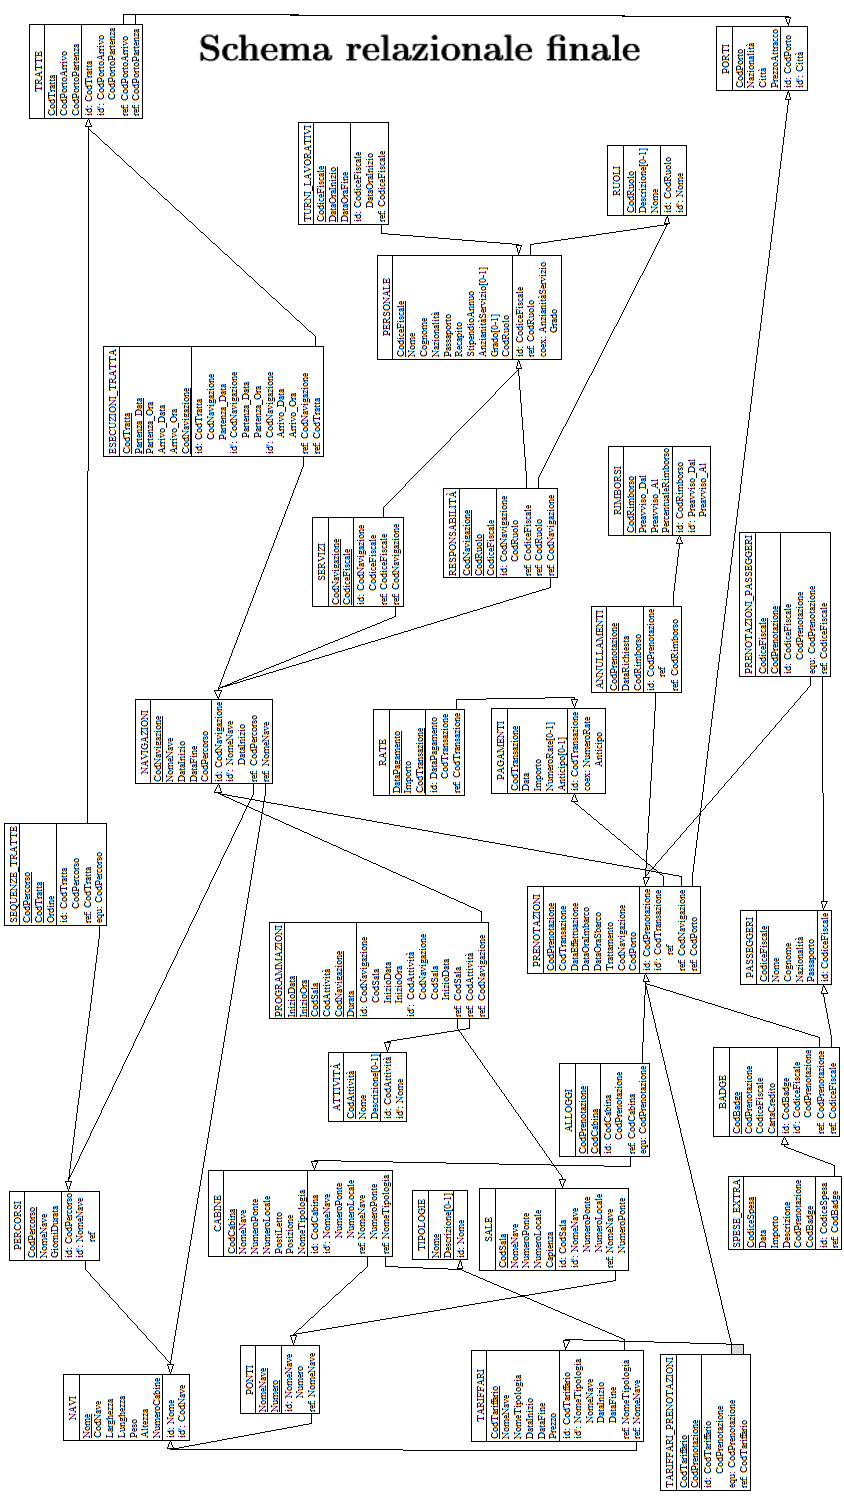
\includegraphics[scale=0.78]{images/RelazionaleCompl2.png}
	\end{figure}

\newpage
\section*{\centering {Traduzione delle operazioni in query SQL}}
\addcontentsline{toc}{section}{Traduzione delle operazioni in query SQL}	


\subsection*{Operazione 1: Inserimento di una prenotazione}
Prima dell'inserimento, viene verificato che il passeggero non sia già presente in un altra prenotazione nello stesso periodo
\begin{lstlisting}
SELECT COUNT(*)
FROM PRENOTAZIONI_PASSEGGERI PS, PRENOTAZIONI P
WHERE PS.CodiceFiscale = <CF passeggero>
AND P.CodPrenotazione = PS.CodPrenotazione
AND DataOraImbarco BETWEEN P.DataOraImbarco AND P.DataOraSbarco
OR DataOraSbarco BETWEEN P.DataOraImbarco AND P.DataOraSbarco
\end{lstlisting}
Se l'esito della query restituisce 0 tuple, allora si può procedere all'inserimento del passeggero con le due query seguenti

\begin{lstlisting}
INSERT INTO PASSEGGERI(CodiceFiscale,Nome,Cognome,Nazionalità,Passaporto)
VALUES(??, ??, ...)
\end{lstlisting}

\begin{lstlisting}
INSERT INTO PRENOTAZIONI_PASSEGGERI(CodiceFiscale,CodPrenotazione)
VALUES(??, ??, ...)
\end{lstlisting}

Inserimento del badge associato a ciascun passeggero
\begin{lstlisting}
INSERT INTO BADGE(CodBadge,CodPrenotazione,CodiceFiscale,CartaCredito)
VALUES(??, ??, ...)
\end{lstlisting}

Inserimento della prenotazione
\begin{lstlisting}
INSERT INTO PRENOTAZIONI(CodPrenotazione,CodTransazione,DataEffettuazione,DataOraImbarco,
                            DataOraSbarco,Trattamento,CodNavigazione,CodPorto)
VALUES(??, ??, ...)
\end{lstlisting}

Selezione delle cabine disponibili avendo selezionato tramite applicativo <nome nave>, <CodNavigazione>, <DataOraImbarco>, <DataOraSbarco>, <tipologia cabina> e <posizione cabina>
\begin{lstlisting}
SELECT C1.CodCabina
FROM CABINE C1
WHERE C1.NomeNave = <nome nave>

EXCEPT

SELECT C.*
FROM PRENOTAZIONI P,ALLOGGI A, CABINE C
WHERE P.CodNavigazione = <CodNavigazione>
AND P.DataOraImbarco >= <DataOraImbarco>
AND P.DataOraSbarco <= <DataOraSbarco>
AND A.CodPrenotazione = P.CodPrenotazione 
AND C.NomeNave = <nome nave>
AND C.CodCabina = A.CodCabina
AND C.Posizione = <posizione cabina>
AND C.NomeTipologia = <tipologia cabina>
\end{lstlisting}
Una volta selezionate dall'utente poi verranno inserite in ALLOGGI tramite la query:
\begin{lstlisting}
INSERT INTO ALLOGGI(CodPrenotazione,CodCabina)
VALUES(??, ??, ...)
\end{lstlisting}

Considerato <codici Cabina Prenot> come l'insieme dei <codCabina> selezionati fra quelli disponibili, si vanno a reperire tutti i codTariffario dei tariffari applicati alla prenotazione per il calcolo dell'importo di pagamento (da calcolare successivamente)
\begin{lstlisting}
SELECT T.CodTariffario
FROM TARIFFARI T
WHERE T.NomeTipologia IN (SELECT DISTINCT C.NomeTipologia
                    FROM CABINE C
                    WHERE C.CodCabina IN {<codici Cabina Prenot>})
\end{lstlisting}

Inserimento tariffari prenotazioni
\begin{lstlisting}
INSERT INTO TARIFFARI_PRENOTAZIONI(CodTariffario,CodPrenotazione)
VALUES(??, ??, ...)
\end{lstlisting}

Inserimento di un pagamento (dopo aver opportunamente calcolato l'importo in base ai tariffari applicati)
\begin{lstlisting}
INSERT INTO PAGAMENTI(CodTransazione,Data,Importo,NumeroRate,Anticipo)
VALUES(??, ??, ...)
\end{lstlisting}

\subsection*{Operazione 2: Inserimento nuova navigazione}
\begin{lstlisting}
INSERT INTO NAVIGAZIONI(NomeNave, DataInizio, DataFine, CodPercorso)
VALUES(??, ??, ...)
\end{lstlisting}

\vspace{0.5cm}
\subsection*{Operazione 3: Inserimento di una nuova nave}
\begin{lstlisting}
INSERT INTO NAVI(NomeNave, Larghezza, Lunghezza, Peso, Altezza, NumeroCabine)
VALUES(??, ??, ...)
\end{lstlisting}

\vspace{0.5cm}
\subsection*{Operazione 4: Inserimento di Spesa Extra}
\begin{lstlisting}
INSERT INTO SPESE\_EXTRA(NomeNave, Larghezza, Lunghezza, Peso, Altezza, NumeroCabine)
VALUES(??, ??, ...)
\end{lstlisting}

\vspace{0.5cm}
\subsection*{Operazione 5: Visualizzazione delle navigazioni associate ad una nave X}
\begin{lstlisting}
SELECT *
FROM NAVIGAZIONI N
WHERE N.NomeNave = X
\end{lstlisting}

\vspace{0.5cm}
\subsection*{Operazione 6: Visualizzazione dell'esecuzione tratta all'interno di una navigazione X}
\begin{lstlisting}
SELECT *
FROM ESECUZIONI_TRATTE E
WHERE E.CodNavigazione = X
\end{lstlisting}

\vspace{0.5cm}
\subsection*{Operazione 7: Visualizzazione del percorso e delle relative tratte associate ad una nave X}
\begin{lstlisting}
SELECT P.CodPercorso, S.CodTratta, T.CodPortoArrivo, T.CodPortoPartenza
FROM PERCORSI P, SEQUEZE\_TRATTE S, TRATTE T
WHERE P.CodPercorso = S.CodPercorso
AND S.CodTratta = T.CodTratta
AND P.NomeNave = X
\end{lstlisting}

\vspace{0.5cm}
\subsection*{Operazione 8: Visualizzazione della programmazioni relative ad una navigazione}
\begin{lstlisting}
SELECT *
FROM PROGRAMMAZIONI P
WHERE P.CodNavigazione = X
\end{lstlisting}

\newpage
\subsection*{Operazione 9: Visualizzazione delle responsabilità relative ad una navigazione}
\begin{lstlisting}
SELECT P.CodiceFiscale, R.CodRuolo
FROM RESPONSABILITÀ R, PERSONALE P
WHERE P.CodiceFiscale = P.CodiceFiscale
AND R.CodNavigazione = X
\end{lstlisting}

\vspace{0.5cm}
\subsection*{Operazione 10: Visualizzazione dei turni lavorativi di un personale all'interno di una navigazione X}
\begin{lstlisting}
SELECT T.*
FROM SERVIZI S, PERSONALE P, TURNI_LAVORATIVI T, (SELECT * 
                                                  FROM NAVIGAZIONI N 
                                                  WHERE N.CodNavigazione = X) AS NAV
WHERE S.CodNavigazione = NAV.CodNavigazione
AND S.CodiceFiscale = P.CodiceFiscale
AND P.CodiceFiscale = T.CodiceFiscale
AND T.DataOraInizio BETWEEN NAV.DataInizio AND NAV.DataFine
AND T.DataOraFine BETWEEN NAV.DataInizio AND NAV.DataFine
\end{lstlisting}

\vspace{0.5cm}
\subsection*{Operazione 11: Visualizzazione del personale con più responsabilità}
\begin{lstlisting}
SELECT TOP(1) WITH TIES R.CodiceFiscale, P.Nome, P.Cognome, COUNT(*) AS NumResponsabilità
FROM RESPONSABILITÀ R, PERSONALE P
WHERE R.CodiceFiscale = P.CodiceFiscale
GROUP BY R.CodiceFiscale, P.nome, P.Cognome
ORDER BY 4 DESC
\end{lstlisting}

\vspace{0.5cm}
\subsection*{Operazione 12: Percorsi più apprezzati}
\begin{lstlisting}
SELECT N.CodPercorso, COUNT( ) AS NumeroPrenotazioni
FROM PRENOTAZIONI P, NAVIGAZIONI N
WHERE P.CodNavigazione = N.CodNavigazione
AND YEAR(P.DataEffettuazione) = YEAR(GETDATE())
GROUP BY N.CodPercorso
\end{lstlisting}

\vspace{0.5cm}
\subsection*{Operazione 13: Costo medio delle prenotazioni per ciascun percorso}
Calcolato raggruppando per percorso la media degli importi pagati per ciascuna prenotazione
\begin{lstlisting}[]
SELECT N.CodPercors, AVG(PA.Importo) AS ImportoMedio
FROM NAVIGAZIONI N, PAGAMENTI PA, PRENOTAZIONI PR
WHERE N.CodNavigazione = PR.CodNavigazione
AND PA.CodTransazione = PR.CodTransazione
GROUP BY N.CodPercorso
\end{lstlisting}

\newpage
\subsection*{Operazione 14: Incassi lordi dell'ultimo anno}
In questo modo ottengo gli incassi derivanti dalle prenotazioni 
\begin{lstlisting}
SELECT SUM(P.Importo) AS RicaviPrenotazioni
FROM PRENOTAZIONI PR, PAGAMENTI P
WHERE PR.CodTransazione = P.CodTransazione
AND YEAR(P.DataPagamento) = YEAR(GETDATE())
AND PR.CodPrenotazione NOT IN (SELECT A.CodPrenotazione
                               FROM ANNULLAMENTI A)
\end{lstlisting}
Vengono poi considerati gli incassi derivanti dalle spese extra:
\begin{lstlisting}
SELECT SUM(S.Importo) AS RicaviSpeseExtra
FROM SPESE_EXTRA S
WHERE YEAR(S.DataSpesa) = YEAR(GETDATE())
\end{lstlisting}
Infine vengono sommati.

\vspace{0.5cm}
\subsection*{Operazione 15: Porti con più imbarchi}
\begin{lstlisting}
SELECT PO.Città, COUNT(*) AS Imbarchi
FROM PRENOTAZIONI P, PORTI PO
WHERE P.CodPorto = PO.CodPorto
GROUP BY P.CodPorto, PO.Città
ORDER BY 2 DESC
\end{lstlisting}

\vspace{0.5cm}
\subsection*{Operazione 16: Visualizzazione del tariffario di una nave X e tipologia Y}
\begin{lstlisting}
SELECT *
FROM TARIFFARI T
WHERE T.NomeNave = X
AND T.Tipologia = Y
\end{lstlisting}

\vspace{0.5cm}
\subsection*{Operazione 17: Inserimento di un nuovo percorso}
Prima dell'inserimento di un percorso occorre aver prima inserito una sequenza di tratte, nonchè tratte e porti
\begin{lstlisting}
INSERT INTO SEQUENZE_TRATTE(CodPercorso, CodTratta)
VALUES(?, ?),
(?, ?), 
...;

INSERT INTO PERCORSI(CodPercorso, NomeNave, GiorniDurata)
VALUES(?, ?, ?)
\end{lstlisting}

\chapter*{\LARGE {Progettazione dell'applicazione}}
\addcontentsline{toc}{chapter}{Progettazione dell'applicazione}

L'applicazione per interfacciarsi con il database è stata realizzata in C\#, sfruttando le funzionalità offerte da LINQ; il database risiede in locale ed utilizza SQL Server come DBMS. \\

\noindent
All'avvio, l'applicativo mostra cinque pagine, ciascuna corrispondente a un'area semantica del database, nelle quali è possibile sia inserire che opportunamente visionare i dati ammessi. Viene di seguito data un'\textit{overview} generale per ciascuna di queste.\\

\noindent
Nella pagina dedicata alla prenotazioni (\Cref{img:screen-booking}) l'utente può visualizzare in forma tabellare tutte le prenotazioni inserite nel database, ivi comprese quelle annullate, e inserire un nuovo pagamento di rata (uno al giorno per prenotazione). \\

\begin{figure}[h]
\centering{}
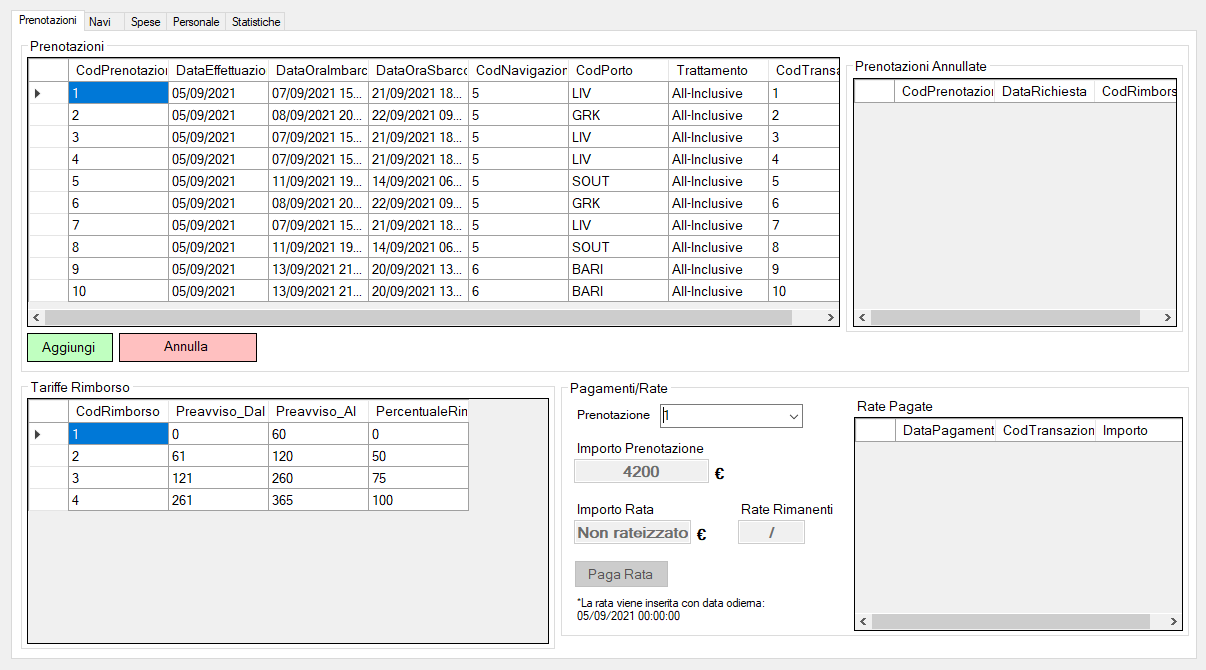
\includegraphics[width=\textwidth]{images/screen-booking.PNG}
\caption{Pagina dedicata alla visualizzazione delle prenotazioni.}
\label{img:screen-booking}
\end{figure}

\noindent
L'inserimento di una nuova prenotazione e di tutti i suoi correlati dati viene demandata ad un apposito form (\Cref{img:insert-booking}). Qui l'utente può scegliere da appositi menù a tendina le informazioni del soggiorno più di suo gradimento per creare la propria prenotazione. Si evidenzia come le scelte dell'utente vengano "accompagnate" in ogni fase dal software, il quale provvede a proporre le sole alternative possibili in conformità dei vincoli analizzati nella fase di progettazione, evitando in questo modo all'utente di poter incorrere in stati non legali o semanticamente non corretti.

\begin{figure}[h]
\centering{}
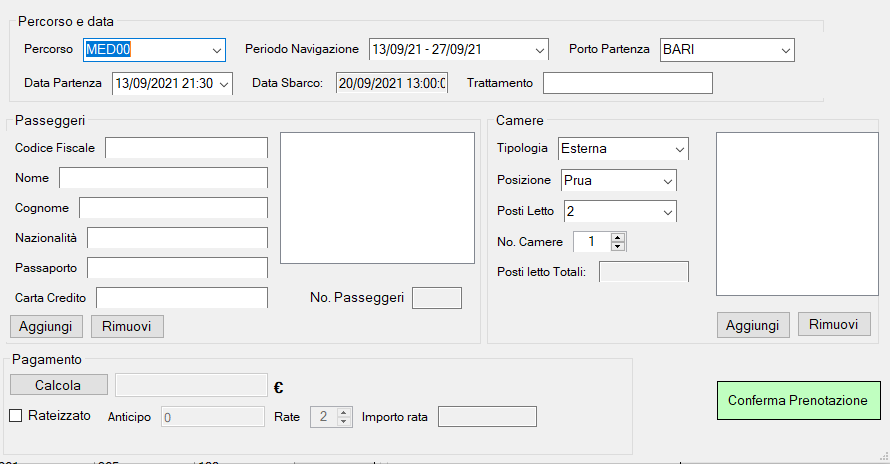
\includegraphics[scale=0.6]{images/screen-insert-booking.PNG}
\caption{Inserimento di una nuova prenotazione.}
\label{img:insert-booking}
\end{figure}

\newpage \noindent
La pagina di visualizzazione delle navi e dei percorsi associate alle stesse offre una visione delle sue caratteristiche principali e del programma di viaggio per una data navigazione, che l'utente liberamente sceglie attraverso un menù a tendina. Cliccando gli appositi pulsanti verranno aperte le maschere per l'inserimento delle navi, dei percorsi e delle tratte eseguite, con tutte le correlate informazioni. Come già detto in precedenza, l'inserimento avviene completando in cascata diversi campi dell'applicazione in modo sia di agevolare l'utente nella scremature delle possibilità di scelta, sia per evitare di imbattersi in stati non ammissibili.

\begin{figure}[h]
\centering{}
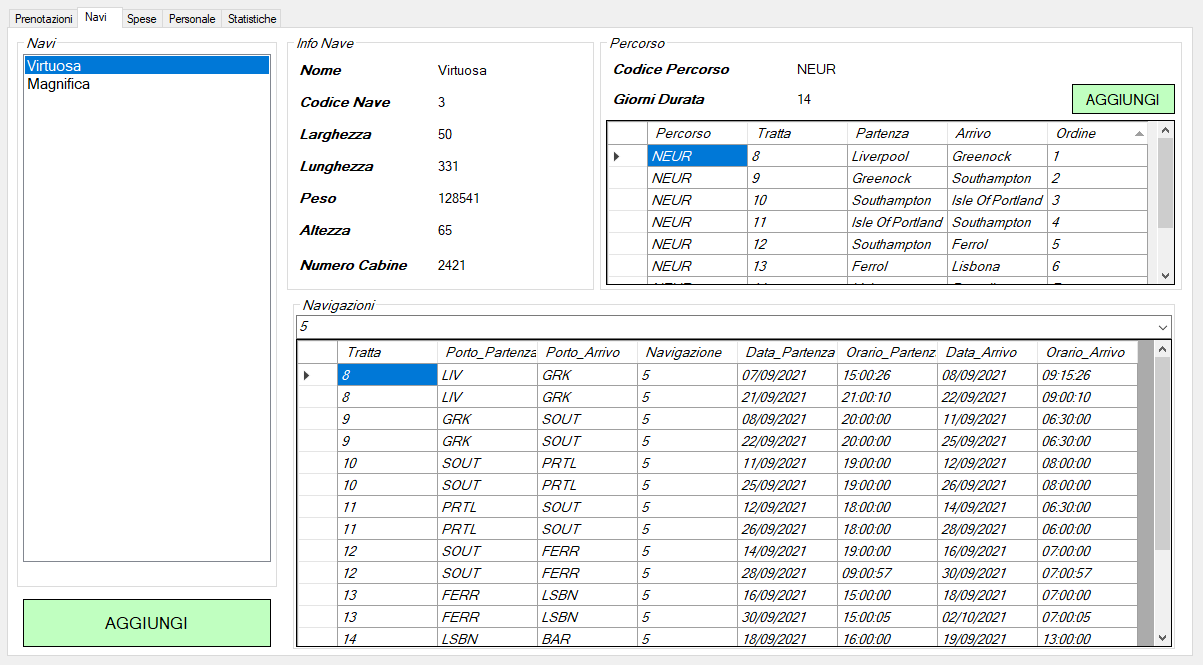
\includegraphics[width=\textwidth]{images/screen-ships.PNG}
\caption{Visualizzazione delle navi e del programma di viaggio per una selezionata navigazione}
\label{img:screen-ships}
\end{figure}

\noindent
Del tutto analoghi ai precedenti i \textit{tab} che riguardano le spese e la gestione del personale di bordo. \\

\noindent
L'ultima pagina è dedicata all'esecuzione e visualizzazione di alcune \textit{query} di tipo statistico circa i dati inseriti all'interno del database. In particolare è data la possibilità all'utente, qualora lo ritenga necessario, di eseguire una o più query di quelle proposte cliccando il relativo bottone e visualizzare a lato, in un istogramma, i dati elencati espressi in forma tabellare a lato.

\begin{figure}[h]
\centering{}
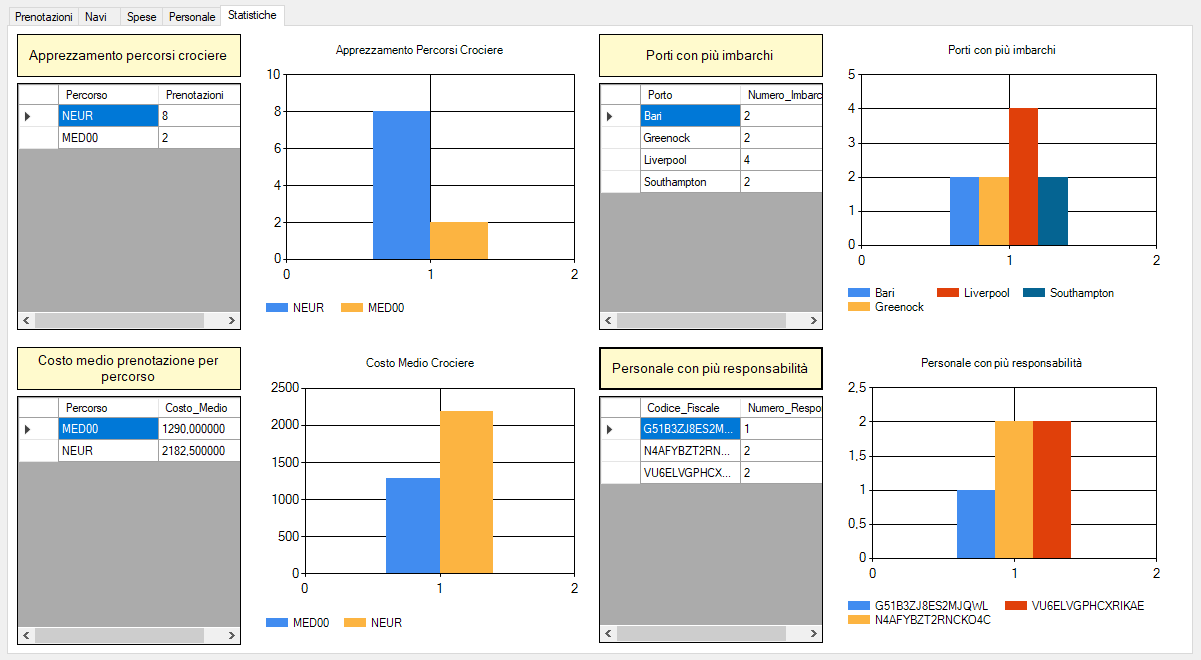
\includegraphics[width=\textwidth]{images/screen-stats.PNG}
\caption{Pagina dedicata alla visualizzazione delle statistiche.}
\label{img:screen-stats}
\end{figure}


\end{document}